%%
%% Main file for ISSTA 2026 submission
%% RAGFlow: Detecting Blockchain Attacks with Fine-grained Trace Knowledge
%%

%%
%% Commands for TeXCount
%TC:macro \cite [option:text,text]
%TC:macro \citep [option:text,text]
%TC:macro \citet [option:text,text]
%TC:envir table 0 1
%TC:envir table* 0 1
%TC:envir tabular [ignore] word
%TC:envir displaymath 0 word
%TC:envir math 0 word
%TC:envir comment 0 0

%% For submission and review
%\documentclass[acmsmall,screen,review,anonymous,nonacm]{acmart}
\documentclass[acmsmall,screen,review,anonymous]{acmart}
%% Note: Use XeLaTeX for compilation

%%% Additional packages
%\usepackage[most]{tcolorbox}
%\usepackage{array}
%\usepackage{booktabs}
%
%%% siunitx commented out - not available in this TeX environment
%%\usepackage{siunitx}
%%\sisetup{detect-weight=true, detect-family=true, table-number-alignment=center}
%
%\usepackage{caption}
%\usepackage{multirow}
%\usepackage{makecell}
%%\usepackage{siunitx} % Commented out - not available
%\usepackage{enumitem}
%\usepackage{pifont}
%\usepackage{ragged2e}
%\usepackage{tabularx}
%\usepackage{xspace}
%%% macros.tex
%%% Import packages, define utility commands and define macros
%%% Version 1.1.0

%%%----------
%%% Imports

%%% Text Formatting
\usepackage{xspace}
\usepackage{xcolor}
\usepackage{graphicx}
\usepackage[normalem]{ulem} % normalem do not replace \emph to underline
%\usepackage{amsmath, amssymb, amsfonts}
\usepackage{enumitem}
\usepackage{microtype}
\usepackage{hyphenat}
%%% Reference, Citation and Link
%\usepackage[hyphens]{url}
%\usepackage{url}
%\usepackage[hidelinks]{hyperref}
%\usepackage[hyphens]{url}
\usepackage[anythingbreaks]{breakurl}
%\usepackage{cite}

%%% Tables
\usepackage{booktabs}
\usepackage{multirow}
\usepackage{makecell}
\usepackage{ragged2e}
\usepackage{longtable}
\usepackage{diagbox}
%%% Plots
\usepackage{caption}
% \usepackage{subcaption}
\usepackage{subfloat}
% \usepackage{subfig}
\usepackage[caption=false]{subfig}
\usepackage{wrapfig}
% Code
\usepackage{listings}

%\usepackage[margin=25mm, a4paper, showframe]{geometry}
\usepackage[many]{tcolorbox}
\usepackage{lipsum}

% Proof
\usepackage{bussproofs}
\usepackage{stackengine}

% Tikz Figs
\usepackage{pifont}
\usepackage{tikz}
%\usepackage{pgf-umlsd} % for flow diagram
\usetikzlibrary{calc}
\usetikzlibrary{shapes.geometric}
\usetikzlibrary{decorations.pathreplacing}
\usetikzlibrary{positioning}
\usetikzlibrary{calc}
\usetikzlibrary{arrows}
\usetikzlibrary{shadows}
%\usetikzlibrary{shapes}

%%% Miscellaneous
\usepackage{balance}
%\usepackage{flushend} % balance the end of double column document
\usepackage{datetime} % for getting current date time

% Algorithm
% \usepackage{algorithm}
% \usepackage{algpseudocode}
% % Define custom Input/Output keywords
% \renewcommand{\algorithmicrequire}{\textbf{Input:}}
% \renewcommand{\algorithmicensure}{\textbf{Output:}}

\usepackage[ruled,vlined,linesnumbered]{algorithm2e}
\SetKw{Return}{return}

\usepackage[capitalize]{cleveref}
\crefname{section}{Sect.}{Sects.}
\Crefname{section}{Section}{Sections}

%%%----------
%%% Utility Commands
%\renewcommand\footnotetextcopyrightpermission[1]{}
%\settopmatter{printacmref=false}

\setlength{\abovedisplayskip}{5pt}
\setlength{\belowdisplayskip}{5pt}
\setlength{\abovecaptionskip}{5pt}
\setlength{\belowcaptionskip}{5pt}
\setlength{\textfloatsep}{5pt}
\setlength{\floatsep}{5pt}
\setlength{\intextsep}{5pt}
\setlength{\dbltextfloatsep}{5pt}
\setlength{\dblfloatsep}{5pt}

\newcommand{\XSpace}[1]{}
\newcommand{\XComment}[1]{}
\newcommand{\liu}[1]{\textcolor{red}{Liu Ye: #1}}
\newcommand{\Fix}[1]{\textcolor{red}{#1}}
\newcommand{\Blue}[1]{\textcolor{blue}{#1}}


\DeclareMathOperator*{\argmax}{arg\,max}
\newcommand{\tool}{\textsc{TxShield}\xspace}


%code block style
\newcommand{\red}[1]{\textcolor[rgb]{1.00,0.00,0.00}{#1}}
\newcommand{\blue}[1]{\textcolor[rgb]{0.00,0.00,1.00}{#1}}
\newcommand{\green}[1]{\textcolor[rgb]{0.00,0.60,0.00}{#1}}
\newcommand{\darkblue}[1]{\textcolor[rgb]{0.00,0.00,0.65}{#1}}
\newcommand{\darkred}[1]{\textcolor[RGB]{139,0,0}{#1}}
\newcommand{\lightred}[1]{\textcolor[RGB]{255,204,203}{#1}}
\newcommand{\myred}[1]{\textcolor[rgb]{1.00,0.00,0.00}{#1}}

\definecolor{silver}{RGB}{192,192,192}
\newcommand{\HighlightCode}[1]{\hspace{-3pt}\colorbox{silver}{#1\vphantom{-}}}

% for table headers
\newcommand{\specialcell}[2][c]{%
  \begin{tabular}[#1]{@{}c@{}}#2\end{tabular}}
\newcolumntype{R}[1]{>{\RaggedLeft\arraybackslash}p{#1}}
\newcolumntype{L}[1]{>{\RaggedRight\arraybackslash}p{#1}}

\newcommand{\cmark}{\ding{51}}
\newcommand{\xmark}{\ding{55}}

%\input{defs-logic} % for logic symbols
%\input{defs-code} % for code listings

% for including revision info in the document
\newcommand{\RevisionInfo}{\Fix{Time: \today{} at \currenttime{.}}}


%%%----------
%%% Macros
%\newcommand{\UPPERCASE}{Title Case\xspace}
%\newcommand{\Firstcap}{First cap\xspace}
%\newcommand{\lowercase}{lower case\xspace}

\newcommand{\MCr}{Maven Central repository\xspace}
\newcommand{\MCR}{Maven Central Repository\xspace}
\newcommand{\github}{GitHub\xspace}
%\newcommand{\stackoverflow}{StackOverflow\xspace}

\newcommand{\df}{differential fact\xspace}
\newcommand{\dfs}{differential facts\xspace}
\newcommand{\old}{original\xspace}
\newcommand{\new}{upgraded\xspace}
\newcommand{\Old}{Original\xspace}
\newcommand{\New}{Upgraded\xspace}
\newcommand{\grok}{Grok\xspace}
\newcommand{\evosuite}{\textsc{EvoSuite}\xspace}
\newcommand{\lib}{library\xspace}
\newcommand{\Lib}{Library\xspace}
\newcommand{\client}{client\xspace}
\newcommand{\Client}{Client\xspace}
\newcommand{\difffacts}{inter-version facts\xspace}
\newcommand{\depsfacts}{intra-version facts\xspace}
\newcommand{\cslicer}{\textsc{CSlicer}\xspace}
\newcommand{\definer}{\textsc{Definer}\xspace}
\newcommand{\clltuple}{$\langle cli,$\allowbreak$lib,$\allowbreak$lib'\rangle$\xspace}
\newcommand{\bcel}{Apache BCEL\xspace}
\newcommand{\compatibilitytesting}{upgrade compatibility checking\xspace}
\newcommand{\CompatibilityTesting}{Upgrade Compatibility Checking\xspace}
\newcommand{\oldlibsym}{$lib$\xspace}
\newcommand{\newlibsym}{$lib'$\xspace}
\newcommand{\clientsym}{$cli$\xspace}

\newcommand{\NumOfSlicingSubjects}{10\xspace}
\newcommand{\dosc}{\textsc{DoSC}\xspace}
\newcommand{\setoftests}{set of tests\xspace}
\newcommand{\NumOfSlicingProjects}{eight\xspace}

\newcommand{\NumOfSubjectsInRTSDataset}{408\xspace}
\newcommand{\NumOfCompatSubjects}{ten\xspace}
\newcommand{\NumOfSubjectsHaveCompatIssues}{four\xspace}
\newcommand{\NumOfSubjectsNotHaveCompatIssues}{six\xspace}
\newcommand{\MaxReduce}{99.11\%\xspace}
\newcommand{\MinReduce}{27.37\%\xspace}

%% Tables
%Symbols for relations
\newcommand{\rCov}{\ensuremath{\mathit{Cov}}\xspace}
\newcommand{\rIns}{\ensuremath{\mathit{Ins}}\xspace}
\newcommand{\rUpd}{\ensuremath{\mathit{Upd}}\xspace}
\newcommand{\rDel}{\ensuremath{\mathit{Del}}\xspace}
\newcommand{\rCall}{\ensuremath{\mathit{Call}}\xspace}
\newcommand{\rRef}{\ensuremath{\mathit{Ref}}\xspace}
\newcommand{\rContain}{\ensuremath{\mathit{Contain}}\xspace}
\newcommand{\rParent}{\ensuremath{\mathit{Parent}}\xspace}
\newcommand{\rHunk}{\ensuremath{\mathit{Hunk}}\xspace}
\newcommand{\rCmt}{\ensuremath{\mathit{Cmt}}\xspace}

% Compat Subjects Table
\newcommand{\TableCaptionCompatSubjects}{Subjects of \CompatibilityTesting Experiment (All URLs Start with https://github.com/)\label{tab:compat:subjects}}
\newcommand{\TableHeadSubjectId}{\textbf{ID}}
\newcommand{\TableHeadClient}{\textbf{Client}}
\newcommand{\TableHeadLib}{\textbf{Library}}
\newcommand{\TableHeadSHA}{\textbf{SHA}}
\newcommand{\TableHeadURL}{\textbf{URL}}
\newcommand{\TableHeadLibOldVer}{\textbf{$Lib$ Version}}
\newcommand{\TableHeadLibNewVer}{\textbf{$Lib'$ Version}}

% Compat Results Table
%% \newcommand{\TableCaptionCompatResults}{Results of Compatibility Testing Experiment (\#CC=the Number of Client Classes; \#QC=the Number of Client Classes Influenced by the Upgrade, obtained by querying Factbase; \%Red=Reduction Rate=(\#CC-\#QC)/\#CC; \#T=the Number of Generated Test Classes; \#FT=the Number of Generated Test Classes that Flip from Pass to Fail after \Lib Upgrade)\label{tab:compat:results}}
\newcommand{\TableCaptionCompatResults}{Results of \CompatibilityTesting Experiment\label{tab:compat:results}}
\newcommand{\TableHeadNumOfAllClasses}{\textbf{\#CC}}
\newcommand{\TableHeadNumOfAffectedClasses}{\textbf{\#AC}}
\newcommand{\TableHeadReduction}{\textbf{\%Reduction}}
\newcommand{\TableHeadNumOfGeneratedTestClasses}{\textbf{\#T}}
\newcommand{\TableHeadNumOfFailedTestClasses}{\textbf{\#FT}}

%% Numbers

%\input{tables/icse2020-compat-subjects-numbers}
%\input{tables/icse2020-compat-result-numbers}

%%%----------
%%% Package settings

% code listing style
\lstdefinestyle{tafile}{%
    basicstyle=\scriptsize\ttfamily,
    %basicstyle=\large,
    frame=single,
    rulecolor=\color{black},
    morekeywords={\$INHERIT, Update, Insert, Delete, reference, contain, call, HunkDep, Coverage},
    tabsize=2,
    numbers=left,                    % where to put the line-numbers; possible values are (none, left, right)
    numbersep=5pt,                   % how far the line-numbers are from the code
    stepnumber=1,
    numberstyle=\tiny\color{gray},   % the style that is used for the line-numbers
    keywordstyle=\sffamily,
}

\lstdefinestyle{syntax}{%
    basicstyle=\small\ttfamily,
    backgroundcolor=\color{white},
    escapeinside={(*}{*)},
    frame=none,
    morekeywords={,id,bid,valuation,allocation,price,max,argmax,}
    tabsize=2,
    numbers=none,                    % where to put the line-numbers; possible values are (none, left, right)
    keywordstyle=\bfseries\color{black}\sffamily,
}
%%% rq box
\newtcolorbox{rqbox}[1]{%
    tikznode boxed title,
    enhanced,
    arc=0mm,
    boxrule=0.5pt,
    interior style={white},
    attach boxed title to top center= {yshift=-\tcboxedtitleheight/2},
    colbacktitle=white,coltitle=black,
    boxed title style={size=normal,colframe=white,boxrule=0pt},
    title=\textbf{Answer to }{\textbf{#1}}}
\newcommand{\prefer}{\vartriangle}
\newcommand{\announce}{\triangledown}
\newcommand{\join}{\oplus}
\newcommand{\associate}{\barwedge}
\newcommand{\reduce}{ \mapsto}
\newcommand{\fourspace}{\xspace\xspace\xspace\xspace}
\newcommand{\twospace}{\xspace\xspace}
\newcommand{\terminate}{\Gamma}
\newcommand{\expand}{::=}
\newcommand{\N}{\mathbb{N}}
\newcommand{\R}{\mathbb{R}}
\newcommand{\Octon}{\mathbb{O}}
\newcommand{\Z}{\mathbb{Z}}
%\hypersetup{draft}

\definecolor{codegreen}{rgb}{0,0.6,0}
\definecolor{codegray}{rgb}{0.5,0.5,0.5}
\definecolor{codepurple}{rgb}{0.58,0,0.82}
\definecolor{backcolour}{rgb}{0.95,0.95,0.92}

\lstdefinestyle{mystyle}{
    backgroundcolor=\color{backcolour},
    commentstyle=\color{codegreen},
    keywordstyle=\color{magenta},
    numberstyle=\tiny\color{codegray},
    stringstyle=\color{codepurple},
    basicstyle=\ttfamily\footnotesize,
    breakatwhitespace=false,
    breaklines=true,
    captionpos=b,
    keepspaces=true,
    numbers=left,
    numbersep=5pt,
    showspaces=false,
    showstringspaces=false,
    showtabs=false,
    tabsize=2
}
\lstset{style=mystyle}

\usepackage{alphabeta}
\newcommand{\ra}[1]{\renewcommand{\arraystretch}{#1}}
\usepackage[group-separator={,}]{siunitx}

%% Promptbox no longer needed - using PDF figures instead

%% BibTeX command
\AtBeginDocument{%
  \providecommand\BibTeX{{%
    Bib\TeX}}}

%% Rights management information (to be updated)
\setcopyright{acmlicensed}
\copyrightyear{2026}
\acmYear{2026}
\acmDOI{XXXXXXX.XXXXXXX}

%% Conference information (to be updated for ISSTA 2026)
\acmConference[ISSTA '26]{ACM SIGSOFT International Symposium on Software Testing and Analysis}{July 2026}{TBD}
\acmISBN{978-1-4503-XXXX-X/2026/07}


% 
% Author list
% Ye Liu, Beijing Institute of Technology, liuye5@live.com
% Shiya Li, Wuhan University, 
% Mu.., Wuhan University,
% Wei Ma, Singapore Management University, weima@smu.edu.sg
% Cong Wu, Wuhan 
% Jing Chen, Wuhan University
% Zijian Zhang, Beijing Institute of Technology, zhangzijian@bit.edu.cn
%
%% Custom commands for easy renaming
\newcommand{\approach}{\textsc{TxShield}\xspace}
\newcommand{\dsystem}{DeFiAttackBench\xspace}
\newcommand{\done}{PriceAttackBench\xspace}

%% Document begins
%%
\begin{document}

%% Title
%\title{Detecting Blockchain Attacks with Fine-grained Trace Knowledge}

\title{TxShield: Transaction-level RAG-enabled DeFi Attack Detection}

%% Authors (anonymized for submission)
\author{Anonymous Author(s)}
\affiliation{%
  \institution{Anonymous Institution}
  \country{}}

\renewcommand{\shortauthors}{Anonymous}

%% Abstract
%% Abstract section

\begin{abstract}
Decentralized Finance (DeFi) protocols have become prime targets for sophisticated attacks, with losses exceeding \$3.4 billion in 2025. Existing detection approaches face fundamental limitations: static analyzers cannot capture runtime behaviors, rule-based detectors fail on custom pricing mechanisms, and standalone LLMs suffer from knowledge staleness and hallucinations. We observe that DeFi attacks, despite diverse implementations, exhibit recurring behavioral patterns at the semantic level, suggesting that their apparent diversity masks a small number of underlying semantic structures.

We present \approach, a Retrieval-Augmented Generation framework for real-time DeFi attack detection. \approach constructs an incrementally expandable knowledge base of historical attacks with LLM-generated behavioral summaries, employs a two-stage retrieval mechanism with dynamic similarity thresholding to ensure high-precision context, and applies adaptive prompting to guide LLM reasoning by analogy with retrieved patterns.

Evaluated on 728 transactions spanning 110+ attack types, \approach achieves an F1-score of 0.824, outperforming the state-of-the-art TrxGNNBERT (F1: 0.766) while providing 20$\times$ faster detection. On price manipulation benchmarks, \approach attains 95.60\% recall compared to 80.22\% for DeFiScope. Ablation studies confirm that the RAG framework contributes 0.586 absolute F1 improvement over vanilla LLM. \approach demonstrates that leveraging historical attack knowledge enables effective detection of novel attacks sharing behavioral semantics with known patterns.
\end{abstract}


%% CCS Concepts (to be updated)
\begin{CCSXML}
<ccs2012>
 <concept>
  <concept_id>10011007.10011074.10011099.10011102.10011103</concept_id>
  <concept_desc>Software and its engineering~Software testing and debugging</concept_desc>
  <concept_significance>500</concept_significance>
 </concept>
 <concept>
  <concept_id>10002978.10003022.10003023</concept_id>
  <concept_desc>Security and privacy~Software security engineering</concept_desc>
  <concept_significance>500</concept_significance>
 </concept>
</ccs2012>
\end{CCSXML}

\ccsdesc[500]{Software and its engineering~Software testing and debugging}
\ccsdesc[500]{Security and privacy~Software security engineering}

%% Keywords
\keywords{Smart Contract Security, DeFi Attack Detection, Retrieval-Augmented Generation, Transaction Analysis, Blockchain Security}

%% Teaser figure (optional, comment out if not needed)
% \begin{teaserfigure}
%   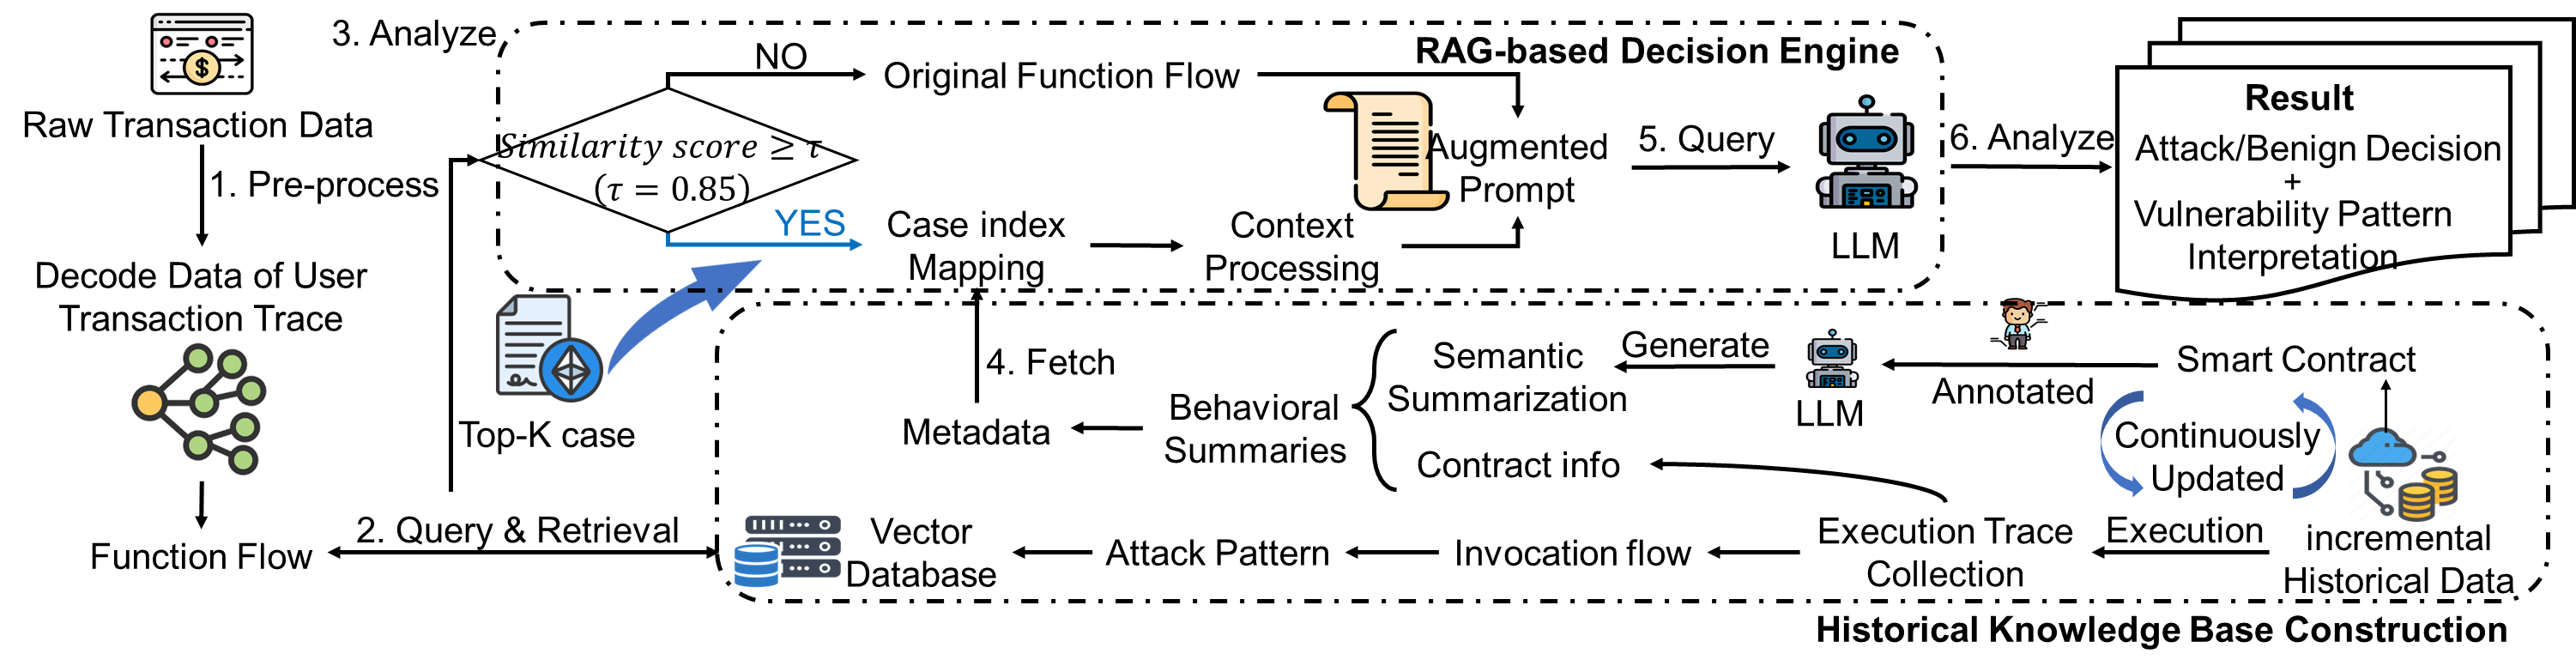
\includegraphics[width=\textwidth]{pic/flowchart2.png}
%   \caption{A high-level overview of RAGFlow}
%   \Description{Overview of the RAGFlow system architecture}
%   \label{fig:teaser}
% \end{teaserfigure}

\maketitle

%% Main content sections
%% Introduction section

\section{Introduction}
\label{sec:introduction}
% P1: Problem Context - The rise of DeFi and security challenges
Decentralized Finance (DeFi) has emerged as a major application of blockchain technology, enabling permissionless financial services through smart contracts.
By late 2025, the total value locked (TVL) in DeFi protocols had exceeded \$230 billion, reflecting the substantial financial value managed by DeFi systems~\cite{defiTVL2025}.
This rapid growth has attracted a large user base, with tens of millions of users interacting with DeFi protocols worldwide.
The increasing scale of DeFi has been accompanied by significant security challenges.
Industry analyses report that losses from cryptocurrency hacks and exploits exceeded \$3.4 billion in 2025, with DeFi protocols representing a major attack surface~\cite{cryptoLoss2025,chainalysis2025report}.
These attacks span both traditional smart-contract vulnerabilities, such as reentrancy as seen in the DAO incident, and advanced economic exploits that leverage flash loans to manipulate prices and protocol states within a single transaction~\cite{qin2020flashloan}.
The immutable nature of smart contracts exacerbates these risks.
Once deployed, vulnerabilities cannot be patched retroactively, making effective testing and continuous post-deployment monitoring critical for mitigating security threats in DeFi systems.
 

% P2: Limitations of existing approaches
Existing approaches to smart contract security can be broadly categorized into four paradigms, each with inherent limitations. \textit{Static analysis tools} such as Slither~\cite{slither} and Mythril~\cite{mythril2018} use pattern matching and symbolic execution to identify known vulnerability patterns. While effective at detecting classic bugs such as reentrancy, these tools suffer from path explosion in complex contracts and often struggle to capture runtime behaviors or cross-protocol interactions arising from DeFi composability~\cite{defi2023}. \textit{Formal verification frameworks} like Certora Prover~\cite{certoraProver} and KEVM~\cite{Hildenbrandt2018KEVM} provide mathematical guarantees but require substantial manual effort to specify invariants and often struggle to model the dynamic, multi-protocol nature of DeFi. \textit{Rule-based dynamic detection tools} such as DeFiRanger~\cite{defiranger2021}, DeFiTainter~\cite{defitainter2023}, and DeFort~\cite{defort2024} analyze transaction traces to detect price-manipulation attacks. However, these approaches rely on predefined mathematical models of specific pricing mechanisms (e.g., constant-product AMMs), making them less effective for custom protocols with non-standard price models; DeFiScope reports that such custom price models account for 44.2\% of 95 real-world price manipulation attacks collected over the past three years~\cite{zhong2025detectingvariousdefiprice}. \textit{LLM-based approaches} represent a recent paradigm shift. TrxGNNBERT~\cite{TrxGNNBERT} leverages a graph-transformer language model to learn trace-level representations for DeFi fraud detection, while GPTScan~\cite{GPTScan} combines GPT with static analysis for logic-vulnerability detection and iAudit~\cite{iaudit2025} employs fine-tuned models with multi-agent debate for source-code auditing. However, these methods either focus primarily on pre-deployment source-code analysis and cannot detect runtime attacks, or incur high end-to-end overhead for trace construction and model inference, limiting practicality for real-time monitoring. 
LLM hallucinations can lead to plausible but incorrect vulnerability reports.
Moreover, parametric knowledge quickly becomes outdated as attack patterns evolve.
%They also suffer from LLM hallucinations---producing plausible but incorrect vulnerability reports---and from knowledge staleness, since parametric knowledge cannot adapt to rapidly evolving attack patterns without costly retraining.

% P3: Key Insight and Challenges
Our key insight, distilled from years of practical experience in smart-contract security, is that DeFi attacks, despite their diverse manifestations, often exhibit recurring behavioral patterns at the semantic level. For example, a price manipulation attack typically follows a ``borrow, manipulate, and profit'' sequence: obtaining large capital via flash loans, executing trades that artificially inflate or deflate token prices, and extracting profit before repaying the loan, all within a single atomic transaction. This observation suggests that historical attack cases, annotated with behavioral semantics, can serve as a valuable knowledge source to guide the detection of new attacks. 
To empirically ground this insight, we analyze approximately 200 real-world DeFi attack incidents from DeFiHackLabs~\cite{defihacklabs2024}.
Despite their apparent diversity, these attacks consistently fall into eight major semantic categories, with Business Logic Flaws, Price Manipulation, and Reentrancy-based call attacks dominating the incident landscape.
%To empirically substantiate this insight, we analyze about 200 real-world attack incidents from DeFiHackLabs~\cite{defihacklabs2024} and find that these attacks cluster into eight major categories. The top three categories (Business Logic Flaws, Price Manipulation, and Reentrancy \& Call Attacks) account for the majority of all incidents. 
These results provide quantitative evidence that attack patterns are reusable across different protocols.

However, realizing this insight poses three technical challenges: \textbf{(C1) Semantic Gap:} Raw execution traces consist of low-level EVM operations and function calls that are difficult to interpret. \textit{How can we bridge the gap between low-level traces and high-level attack semantics?} \textbf{(C2) Retrieval Precision:} Na\"ive similarity search may retrieve irrelevant or misleading historical cases, introducing noise that can degrade detection accuracy. \textit{How can we ensure that retrieved cases are truly relevant to the query transaction?} \textbf{(C3) Reasoning Reliability:} Even with relevant context, LLMs may hallucinate or fail to correctly apply retrieved knowledge. \textit{How can we guide the LLM to make reliable attack-or-benign decisions?}

% P4: Our Approach
To address these challenges, we propose \approach, a Retrieval-Augmented Generation framework for the DeFi transaction attack detection. At a high level, \approach{} comprises two main components: a \textit{Historical Knowledge Base} and a \textit{RAG-based Decision Engine}. For \textbf{C1}, we construct an incrementally expandable knowledge base by collecting execution traces from historical attack incidents, extracting behavioral summaries using LLM-based semantic summarization, and storing them as vector embeddings alongside structured metadata. This transforms opaque execution traces into interpretable attack patterns. For \textbf{C2}, we design a two-stage retrieval mechanism: the first stage performs vector similarity search to retrieve top-$k$ candidate cases; the second stage applies a dynamic similarity threshold ($\tau = 0.85$) to filter out low-confidence matches, ensuring that only highly relevant cases are used as context. For \textbf{C3}, we employ an adaptive prompting strategy: when high-similarity historical cases exist, we construct an augmented prompt that instructs the LLM to reason by analogy with the retrieved attack patterns; otherwise, the system falls back to zero-shot analysis based solely on the transaction data. This design enables \approach{} to leverage historical knowledge when available while maintaining detection capability for novel attack patterns.

% P5: Results Summary
We evaluate \approach{} on two datasets: \dsystem{}, comprising 728 transactions (364 attacks across 110+ attack types and 364 benign transactions) curated from DeFiHackLabs, and \done{}, a specialized benchmark of 95 price-manipulation attacks~\cite{zhong2025detectingvariousdefiprice}. On \dsystem{}, \approach{} achieves an F1 score of 0.824 with a 15-second average latency, significantly outperforming TrxGNNBERT~\cite{TrxGNNBERT} (F1: 0.766, latency: $\sim$5 minutes). On \done{}, \approach{} attains 95.60\% recall, surpassing DeFiScope (80.22\%), DeFort (54.95\%), and DeFiRanger (52.75\%) by substantial margins. Ablation studies confirm that the RAG framework contributes an absolute F1 gain of 0.586 over a vanilla LLM, while the two-stage retrieval mechanism adds 0.030. Furthermore, \approach{} demonstrates cost efficiency: processing the entire \dsystem{} dataset costs only \$3.86 with GPT-4.1-mini or \$0.26 with Llama-3.1-8B-Instruct.

% P6: Contributions
This paper makes the following contributions:
\begin{itemize}
    \item We present \approach, the first RAG-based framework for the DeFi transaction attack detection that leverages historical attack knowledge to enhance LLM reasoning, addressing the limitations of both rule-based and pure LLM approaches.
    \item We design a two-stage retrieval mechanism with dynamic similarity thresholding that balances recall and precision, ensuring high-quality context for LLM-based reasoning while filtering out potentially misleading cases.
    \item We conduct comprehensive experiments on two datasets spanning 110+ attack types, demonstrating that \approach{} achieves state-of-the-art detection performance with significantly lower latency and cost than existing approaches.
    \item We provide an in-depth analysis of \approach{}'s capability boundaries, identifying scenarios where the system excels (e.g., reentrancy, access control) and where it faces challenges (e.g., cryptographic exploits, multi-step cross-contract attacks), offering insights for future research directions.
\end{itemize}

\noindent\textbf{Roadmap.} Section~\ref{sec:background} introduces the background. Section~\ref{sec:approach} details the design of \approach{}, including knowledge base construction, two-stage retrieval, and adaptive prompting. Section~\ref{sec:evaluation} presents our experimental evaluation and ablation studies, Section~\ref{sec:related_work} demonstrate the related work and Section~\ref{sec:conclusion} concludes with limitations and future directions.
%% Background section

\section{Background}
\label{sec:background}

\paragraph{\textbf{Smart Contracts and DeFi Ecosystem}}
Smart contracts are self-executing programs deployed on blockchain platforms such as Ethereum. Written primarily in Solidity, these contracts are compiled into bytecode and executed by the Ethereum Virtual Machine (EVM), a stack-based virtual machine that processes transactions deterministically across all network nodes. Once deployed, smart contract code is immutable (it cannot be modified or patched), which makes security vulnerabilities particularly consequential.
Decentralized Finance (DeFi) leverages smart contracts to replicate traditional financial services without centralized intermediaries~\cite{defi2023}. The DeFi ecosystem comprises several key protocol types: (1) \textit{Decentralized Exchanges (DEXs)} such as Uniswap~\cite{uniswapv3} enable permissionless token trading through Automated Market Makers (AMMs), where liquidity pools and mathematical formulas (e.g., the constant-product formula $x \cdot y = k$) determine token prices; (2) \textit{Lending Protocols} like Aave~\cite{aaveflashloan} and Compound allow users to lend and borrow assets with interest rates determined algorithmically; and (3) \textit{Flash Loan Providers} offer uncollateralized loans that must be borrowed and repaid within a single atomic transaction~\cite{qin2020flashloan}.
A defining characteristic of DeFi is \textit{composability} (the ability for protocols to interact seamlessly, with outputs from one protocol serving as inputs to another). While composability enables capital efficiency and innovation, it also creates complex attack surfaces where vulnerabilities can span multiple protocols.

\paragraph{\textbf{DeFi Attack Taxonomy}}

%Based on our analysis of 574 real-world attack incidents and existing literature~\cite{defi2023,scvsurvey2024,taxonomysc2024}, we categorize DeFi attacks into the following major types:
Based on existing literature~\cite{defi2023,scvsurvey2024,taxonomysc2024}, we categorize DeFi attacks into the following major types:

\emph{Reentrancy Attacks.} Reentrancy occurs when a contract makes an external call to another contract before updating its own state, allowing the callee to ``re-enter'' the original function and exploit the inconsistent state~\cite{reentrancysurvey2025}. Modern variants include cross-function reentrancy (exploiting state shared across multiple functions) and cross-contract reentrancy (exploiting interactions between multiple contracts)~\cite{blockwatchdog2024,slise2024}.

\emph{Price Manipulation Attacks.} These attacks exploit the mechanism by which DeFi protocols determine asset prices. In AMM-based DEXs, an attacker can execute large trades to temporarily shift the price curve, then exploit this artificial price in another protocol (e.g., a lending platform using the DEX as a price oracle)~\cite{defiranger2021,pomabuster2024}. Flash loans amplify this threat by providing attackers with massive capital at zero upfront cost~\cite{qin2020flashloan}. Time-Weighted Average Price (TWAP) oracles, designed to mitigate single-block manipulation, remain vulnerable to multi-block attacks~\cite{oraclesurvey2023}.

\emph{Access Control Vulnerabilities.} These vulnerabilities arise when privileged functions lack proper authorization checks, allowing unauthorized users to execute administrative operations such as minting tokens, modifying parameters, or draining funds~\cite{GPTScan}. Variants include missing access modifiers, incorrect role assignments, and unprotected initialization functions.

\emph{Business Logic Flaws.} Unlike generic vulnerability patterns, business logic flaws are protocol-specific bugs in the implementation of intended functionality. Examples include incorrect reward calculations, flawed liquidation mechanisms, and improper handling of edge cases. These vulnerabilities are particularly challenging to detect because they require understanding the protocol's intended behavior~\cite{iaudit2025}.

\emph{Other Vulnerabilities.} Additional attack vectors include integer overflow/underflow (largely mitigated by Solidity 0.8+), front-running and sandwich attacks exploiting transaction ordering~\cite{zhou2021flashboys}, and governance attacks manipulating decentralized voting mechanisms.

\paragraph{\textbf{Retrieval-Augmented Generation}}

Retrieval-Augmented Generation (RAG) is a paradigm that enhances LLM capabilities by incorporating external knowledge retrieval~\cite{lewis2021retrievalaugmentedgenerationknowledgeintensivenlp}. Unlike pure parametric models that rely solely on knowledge encoded in their weights during training, RAG systems dynamically retrieve relevant information from external databases to augment the generation process.
A typical RAG architecture consists of three components: (1) a \textit{knowledge base} storing documents as vector embeddings, (2) a \textit{retriever} that identifies relevant documents given a query, and (3) a \textit{generator} (typically an LLM) that produces outputs conditioned on both the query and retrieved context. The retrieval process typically employs dense vector similarity search, where queries and documents are mapped to a shared embedding space and relevance is measured by cosine similarity or other distance metrics.
RAG addresses two fundamental limitations of standalone LLMs. First, it mitigates \textit{knowledge staleness}: while LLM parameters are fixed after training, the knowledge base can be continuously updated with new information. Second, it reduces \textit{hallucination}: by grounding generation in retrieved evidence, RAG systems produce more factually accurate outputs~\cite{llmhallucination2024}. These properties make RAG particularly suitable for domains requiring up-to-date, specialized knowledge, such as detecting rapidly evolving DeFi attack patterns.

%% Approach section

\section{Approach Overview}
\label{sec:approach}
This section presents the design of \approach, a retrieval-augmented framework for real-time DeFi attack detection. We first provide an overview of the system architecture and then detail each component: the historical knowledge base construction pipeline, the two-stage retrieval mechanism, and the adaptive LLM-based reasoning module.

%% Overview figure
\begin{figure*}[htbp]
	\centering
	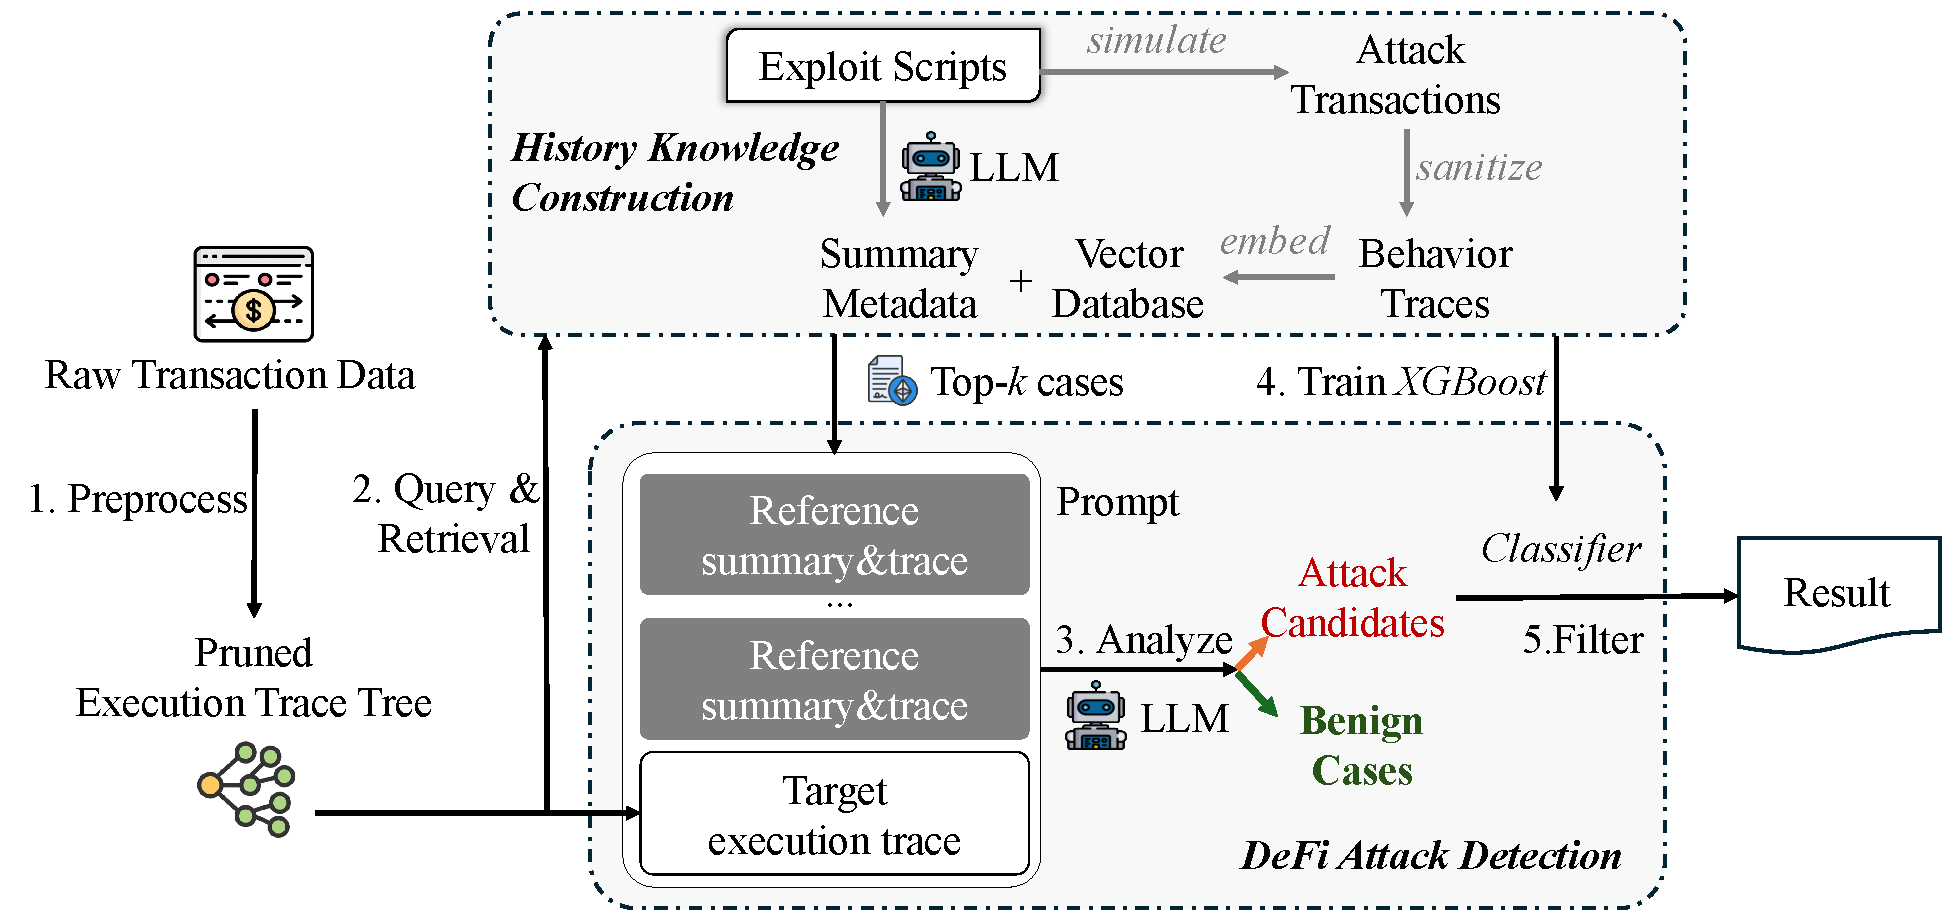
\includegraphics[width=.9\textwidth]{pic/TxHunt.pdf}
	\caption{A high-level overview of \approach}
	\label{fig:flowchart}
\end{figure*}

%\subsection{System Overview}

As illustrated in Figure~\ref{fig:flowchart}, \approach comprises two main components that work in tandem to detect DeFi attacks.

The \textit{Historical Knowledge Base} serves as an external memory that stores structured representations of past attack incidents. Unlike static rule sets, this knowledge base captures behavioral semantics---high-level descriptions of how attacks unfold---enabling \approach{} to recognize novel attack variants that share similar patterns with known incidents. The knowledge base can be incrementally expanded as new attacks are discovered and analyzed.

The \textit{RAG-based Decision Engine} processes incoming transactions through a pipeline that (1) extracts and normalizes execution traces, (2) retrieves relevant historical cases via similarity search, (3) applies a dynamic threshold to filter retrieval results, and (4) constructs prompts that guide an LLM to make attack-versus-benign decisions. The engine adapts its behavior based on retrieval results: when high-similarity historical cases exist, it leverages them for analogical reasoning; otherwise, it falls back to zero-shot analysis.

This architecture addresses the three challenges identified in Section~\ref{sec:introduction}: the knowledge base construction bridges the semantic gap (C1) by transforming low-level traces into interpretable summaries; the two-stage retrieval ensures precision (C2) by filtering out irrelevant or misleading cases; and the adaptive prompting strategy enhances reasoning reliability (C3) by grounding LLM decisions in relevant evidence.

\section{Security Knowledge Construction}
\label{sec:knowledge-base}

The knowledge base construction pipeline transforms raw historical attack data into a searchable repository of behavioral patterns. The constructions encompass three stages: execution trace minimization, semantic summarization, and vector indexing.

% \subsection{Execution Trace Collection}

We source historical attack incidents from DeFiHackLabs~\cite{defihacklabs2024}, a curated repository containing Proof-of-Concept (PoC) implementations of real-world DeFi exploits. To avoid data leakage in our experiments, we randomly sample $\sim$200 incidents to construct the knowledge base and reserve the remaining incidents for evaluation (Section~\ref{sec:evaluation}). Each PoC is a Foundry~\cite{foundry} test case that reproduces the attack on a forked blockchain state. For each incident, we execute the PoC and collect:

\begin{itemize}
    \item Invocation Flow: The sequence of external and internal function calls, including contract addresses, function signatures, and call parameters.
    \item State Changes: Modifications to contract storage, particularly balance changes for relevant tokens.
    \item Event Logs: Emitted events that signal significant operations (e.g., \texttt{Transfer}, \texttt{Swap}, \texttt{Borrow}).
    \item Metadata: Attack date, affected protocol, estimated loss, and attack type labels (when available).
\end{itemize}

The raw trace data captures the very execution details of an attack but often lacks the semantic context needed for effective analysis. 
To eliminate execution noise and reduce the trace size, we apply a minimization algorithm that removes redundant or low-information nodes while preserving the essential control-flow and asset-flow semantics of the attack.

\subsection{Execution Trace Minimization}
Raw execution traces are often complicated and verbose, resulting in overly too large context bases for LLM to reason efficiently and effectively in limited context windows.  
Our investigation reveals that exploit transactions exhibit similar execution patterns. 
First, most of them have manipulated balance of contract accounts, through the operations like \emph{send} or \emph{transfer}.
Second, many of them involve complex contract interactions through external calls, such as \emph{flashloan} that borrows a large amount of tokens from a lending protocol.
With these observations, we devise an algorithm to filter out likely unuseful items within raw execution traces while preserving attack semantics.


\begin{algorithm}[p]
\small
\caption{Execution Trace Tree Minimization}
\label{alg:trace-minimization}
\KwIn{Execution trace tree $\mathcal{T}$ with root $r$; target function
$f_t$; maximum depth $D_{\max}$; maximum argument length $L_{\max}$}
\KwOut{Minimized execution trace tree $\mathcal{T}'$}

$\mathcal{S} \gets \emptyset$\tcp*[r]{Set of previously observed call signatures}
$\textsc{MarkDuplicates}(r,\mathcal{S})$\;

$r' \gets \textsc{GeneralPrune}(r,0,D_{\max},L_{\max})$\;
\If{$r'=\varnothing$}{
    \Return $\emptyset$\;
}

$(P,d_t) \gets \textsc{FindDeepestTarget}(r',f_t)$\; \tcp*[r]{P indicates a deepest call path to the target function $f_t$ at depth $d_t$} \label{func:finddeepest}

\If{$P$ exists}{
    $\textsc{PruneTargetLevel}(r',d_t,f_t)$\; \label{func:prunetarget}
}

\Return the tree rooted at $r'$\;

% \BlankLine
\SetKwFunction{MarkDuplicates}{MarkDuplicates}
\SetKwProg{Fn}{Function}{:}{}

\Fn{\MarkDuplicates{$v,\mathcal{S}$}}{ \label{func:markduplicate:start}
    $\sigma(v) \gets \langle
        v.\mathit{type},
        v.\mathit{contract},
        v.\mathit{function},
        v.\mathit{args},
        v.\mathit{value},
        v.\mathit{return}
	\rangle$\; \label{func:markduplicate:sigma}

    \eIf{$\sigma(v)\in\mathcal{S}$}{
        $v.\mathit{duplicate}\gets\mathsf{true}$\;
    }{
        $\mathcal{S}\gets\mathcal{S}\cup\{\sigma(v)\}$\; \label{func:markduplicate:record}
    }

    \ForEach{$u\in v.\mathit{children}$}{
        $\textsc{MarkDuplicates}(u,\mathcal{S})$\;
    }  \label{func:markduplicate:end}
}

% \BlankLine
\SetKwFunction{GeneralPrune}{GeneralPrune}

\Fn{\GeneralPrune{$v,d,D_{\max},L_{\max}$}}{ \label{func:prune:start}
    \If{$v.\mathit{duplicate}=\mathsf{true}$}{ \label{func:prune:duplicate:start}
        \Return $\varnothing$\;
    } \label{func:prune:duplicate:end}

    \If{$d>D_{\max}$}{
        \Return $\textsc{TruncatedNode}(d)$\; \label{func:prune:truncated}
    }

    \If{$v.\mathit{type}=\texttt{STATICCALL}$ \textbf{and}
        $\textsc{IsMetadataQuery}(v.\mathit{function})$}{ \label{func:prune:metadata:start}
        \Return $\varnothing$\;
    } \label{func:prune:metadata:end}

    $C'\gets\emptyset$\;
    \ForEach{$u\in v.\mathit{children}$}{
        $u'\gets\textsc{GeneralPrune}(u,d+1,D_{\max},L_{\max})$\;
        \If{$u'\neq\varnothing$}{
            $C'\gets C'\mathbin{\|}u'$\;
        }
    }
    $v.\mathit{children}\gets C'$\;

    \If{$|v.\mathit{args}|>L_{\max}$}{ \label{func:prune:length}
        $v.\mathit{args}\gets
        \textsc{Prefix}(v.\mathit{args},L_{\max})
        \mathbin{\|}\texttt{<truncated>}$\;
    }

    $v.\mathit{contract}\gets\textsc{AliasAddress}(v.\mathit{contract})$\; \label{func:prune:alias}
    \Return $v$\; \label{func:prune:end}
}  

% \BlankLine
\SetKwFunction{PruneTargetLevel}{PruneTargetLevel}

\Fn{\PruneTargetLevel{$v,d_t,f_t$}}{ \label{func:prunetarget:start}
    $C'\gets\emptyset$\;
    \ForEach{$u\in v.\mathit{children}$}{
        \If{$u.\mathit{depth}\neq d_t$ \textbf{or}
            $u.\mathit{function}=f_t$}{
            $\textsc{PruneTargetLevel}(u,d_t,f_t)$\;
            $C'\gets C'\mathbin{\|}u$\;
        }
    }
    $v.\mathit{children}\gets C'$\;
} \label{func:prunetarget:end}
\end{algorithm}

% \begin{algorithm}
% 	\caption{Execution Trace Tree Minimization}\label{alg:trace}
% 	\small
% 	\begin{algorithmic}
% 		\Require $\Tau$, \emph{the tree of raw execution trace };\\
% 		\quad \quad $attackFunc$, \emph{the main function of attack script.}
% 		\Ensure $\hat{\Tau}$, \emph{the tree of minimized execution trace.}
% 		\Statex % Empty line for separation 
% 		\Procedure{Remove\_Duplicate}{$\tau$}
% 		\EndProcedure
% 		\Procedure{Prune}{$\tau$}
% 		\EndProcedure
% 		\Procedure{Extract\_Target}{$\tau$}
% 		\EndProcedure
% 		\Procedure{Main}{\Tau}
% 		\State $\hat{\Tau}$ $\gets$ $\emptyset$
% 		\For{$\tau$ in $\Tau$}
% 			\State $\hat{\tau}$ $\gets$ \textsc{Remove\_duplicate}(\tau)
% 			\State $\hat{\tau}$ $\gets$ \textsc{Prune}(\tau)
% 			\State $\hat{\Tau} =  \hat{\Tau} \cup \{\hat{\tau}\}$ 
% 		\EndFor 
% 		\For{$\tau$ in $\hat{\Tau}$}
% 		\If {not \textsc{contain\_Target}(\tau)}
% 			\State $\hat{\Tau} =  \hat{\Tau} \setminus \{\hat{\tau}\}$ 
% 		\EndIf
% 		\EndFor 
% 		\State \textbf{return} $\hat{\Tau}$
				
% 		\EndProcedure
	
% 	\end{algorithmic}
% \end{algorithm}

As shown in Algorithm~\ref{alg:trace-minimization}, the minimization process consists of three stages: duplicate removal, general pruning, and target-oriented pruning.
First, we identify repeated call nodes through a depth-first traversal (Lines~\ref{func:markduplicate:start}-\ref{func:markduplicate:end}). A call is represented by a signature tuple \emph{<type, contract, function, args, value, return>} indicating its call type, contract address, function name, arguments, transferred value, and return value (Line~\ref{func:markduplicate:sigma}). Within each trace tree, only the first occurrence of a signature is retained (Line~\ref{func:markduplicate:record}); subsequent occurrences and their subtrees are removed during pruning stage (Lines~\ref{func:prune:duplicate:start}-\ref{func:prune:duplicate:end}).

Second, we recursively apply general pruning and normalization rules (Lines~\ref{func:prune:start}-\ref{func:prune:end}). Nodes beyond the maximum traversal depth are replaced by truncation markers to preserve the existence of deeper execution while bounding the trace size~(Lines~\ref{func:prune:truncated}). We remove only low-information static metadata queries, namely calls associated with \texttt{decimals}, \texttt{symbol}, and \texttt{name}~(Lines~\ref{func:prune:metadata:start}-\ref{func:prune:metadata:end}). In contrast, other state-dependent queries such as \texttt{balanceOf} and \texttt{getReserves}, as well as event nodes, are retained because they may expose asset-flow or protocol-state evidence. 
Long argument strings are truncated to a fixed length, and contract addresses are converted to compact aliases while preserving their distinguishing prefixes and suffixes (Lines~\ref{func:prune:length}-\ref{func:prune:alias}).

Finally, we perform target-oriented structural pruning if target function(s) are given. After locating the target function \(f_t\), such as \texttt{executeOperation}, we record the depth of its first occurrence (Line~\ref{func:finddeepest}). At that depth, nodes that do not invoke \(f_t\) are removed, whereas nodes at other depths remain subject only to the general pruning rules (Line~\ref{func:prunetarget}, Lines~\ref{func:prunetarget:start}-\ref{func:prunetarget:end}). This step suppresses parallel calls that are less relevant to the monitored execution phase while retaining the context leading to the target call and its nested internal behavior. The resulting minimized tree reduces redundant and low-information content while preserving control-flow, asset-flow, and state-query evidence relevant to attack monitoring.


\subsection{Semantic Summarization and Vector Indexing}

Raw execution traces are verbose and difficult to interpret directly. We use an LLM to generate concise \textit{behavioral summaries} that describe the attack logic in natural language. The summarization prompt instructs the model to:

\begin{enumerate}
    \item Identify the attack type (e.g., price manipulation, reentrancy, access control).
    \item Describe the attack flow in 3--5 steps, focusing on the sequence of operations and their effects.
    \item Highlight key indicators: unusual fund movements, suspicious call patterns, or state manipulation.
    \item Note the vulnerability exploited and how it was triggered.
\end{enumerate}

For example, a flash-loan price manipulation attack might be summarized as: \textit{``The attacker borrows 10~M USDC via an Aave flash loan, swaps to ETH on Uniswap to inflate the ETH/USDC price, deposits ETH as collateral on the victim lending protocol (which uses Uniswap as a price oracle), borrows the maximum amount of USDC against the inflated collateral value, repays the flash loan, and profits \$2.3~M from the price discrepancy.''}
These summaries provide human-readable documentation and, more importantly, distill the semantic essence of attacks into a concise form that offers more useful context for downstream analysis and retrieval.

% \subsection{Vector Indexing}

Each attack case is stored as a record containing: (1) a unique case ID, (2) the behavioral summary, (3) the raw execution trace, and (4) structured metadata. We generate vector embeddings for the behavioral summaries using a pre-trained text embedding model and index them in a vector database.
The vector representation enables semantic similarity search: when a new transaction exhibits patterns similar to known attacks, relevant historical cases can be retrieved even if the specific contracts, function names, or token addresses differ. This ``semantic fingerprinting'' is the foundation of \approach's generalization capability.

\section{In-Context Reasoning for Attack Detection}
\label{sec:retrieval}

Na\"ive similarity search can retrieve cases that are superficially similar but semantically irrelevant, introducing noise that degrades detection accuracy. We design a two-stage retrieval mechanism to ensure high-precision context for LLM reasoning.

\subsection{Knowledge Retrieval}

Given an incoming transaction, \approach{} first preprocesses it to extract the execution trace and generates a query representation. This query is embedded using the same model as the knowledge base, and we perform approximate nearest neighbor search to retrieve the top-$k$ most similar historical cases. We compute pairwise similarity based on the L2 distance in the embedding space: $\text{sim}(q, d) = 1 - \|q - d\|_2$,
%\begin{equation}
%\text{sim}(q, d) = 1 - \|q - d\|_2
%end{equation}
where $q$ is the query embedding and $d$ is a document embedding from the knowledge base. Higher scores indicate greater semantic similarity. We set $k = 5$ to balance recall and computational efficiency.

%\subsubsection{Stage 2: Dynamic Threshold Filtering}

Not all retrieved cases are equally relevant. To filter out low-confidence matches, we apply a similarity threshold $\tau$:
$\mathcal{C}_{\text{filtered}} = \{d_i \in \text{Top-}k \mid \text{sim}(q, d_i) \geq \tau\}$.
%\begin{equation}
%\mathcal{C}_{\text{filtered}} = \{d_i \in \text{Top-}k \mid \text{sim}(q, d_i) \geq \tau\}
%\end{equation}
We empirically set $\tau = 0.85$ based on validation experiments that examined the correlation between similarity scores and detection accuracy. Cases below this threshold are discarded to prevent the LLM from being misled by tangentially related examples.

This two-stage mechanism serves as a ``quality gate'': Stage~1 casts a wide net to capture potentially relevant cases, while Stage~2 refines the results to retain only high-confidence matches. If no cases satisfy the threshold ($\mathcal{C}_{\text{filtered}} = \emptyset$), \approach{} proceeds without retrieval augmentation.

\subsection{Adaptive LLM-Based Reasoning}
\label{sec:reasoning}

The final component leverages an LLM to analyze the transaction and make an attack-versus-benign decision. We employ an adaptive prompting strategy that varies based on the retrieval results.

%\subsubsection{Retrieval-Augmented Prompt}

When closely matching historical cases are retrieved ($\mathcal{C}_{\text{filtered}} \neq \emptyset$), we construct an augmented prompt that includes:

\begin{enumerate}
    \item A \textit{role definition} establishing the LLM as an expert in smart contract attack detection.
    \item The \textit{current transaction}, i.e., the execution trace of the transaction under analysis.
    \item \textit{Historical context}: behavioral summaries and metadata of retrieved cases, with case IDs mapped to detailed security descriptions.
    \item \textit{Analysis instructions} directing the LLM to compare the current transaction against historical patterns, identify shared malicious indicators, and assess the degree of behavioral correspondence.
\end{enumerate}

\begin{figure}[t]
	\begin{tcolorbox}[title=Prompt template for retrieval-augmented detection]
		\emph{Input}:\\
		* Current transaction:  \blue{\{system\_input\}}\\
		* Historical attack examples:  \blue{\{reference\_attack\}}
		\tcbline
		You are an expert in smart contract attack detection. Your task is to analyze the Current transaction against Historical attack examples provided in the context to determine malicious intent.\\
		The historical examples were retrieved due to high behavioral similarity to the current transaction. Therefore, you must assume malicious intent initially and focus on validating the attack pattern.\\
		Following the instructions: \\
		1. Start assuming this is an Attack executing a known pattern. \\
		2. Compare execution flow and fund transfers with historical examples. \\
		3. Ignore function names; focus on operational sequence and security implications.\\
		4. Focus on Inter-contract calls, abnormal fund movements, state manipulation patterns.
		
		\tcbline
		Output MUST begin with a short answer `Attack' or `Benign', followed by below information: \\ 
		1. \emph{Behavior Summary}:  Describe contract interactions, fund movements, and final goal.
		\\
		2. \emph{Comparative Call Sequence Analysis}:  Analyze call sequence. Compare with most similar historical ID(s). State shared malicious steps.\\
		3. \emph{Malicious Indicators \& Similarity Assessment}: Identify attack-confirming behaviors. Rate similarity: High/Moderate/Low. If Benign, provide irrefutable evidence.
	\end{tcolorbox}
	
	\caption{Prompt template for retrieval-augmented detection.}
	\label{fig:prompt1}
\end{figure}


\begin{figure}[t]
	\begin{tcolorbox}[title=Prompt template for zero-shot detection]
		\emph{Input}:\\
		* Current transaction:  \blue{\{system\_input\}}
		\tcbline
		You are an expert in smart contract attack detection. Evaluate whether the current transaction is malicious based only on the provided transaction data.\\
		There is no prior knowledge or historical context provided. Following the instructions: \\
		1. Your judgment must be based purely on the internal logic, security best practices, and execution behavior of the current transaction. \\
		2. Assume the transaction is Benign unless verifiable security flaws or abnormal logic are evident in the input.\\
		\tcbline
		Output MUST begin with a short answer `Attack' or `Benign', followed by below information: \\ 
		1. \emph{Behavior Summary}:  Describe the transaction's overall behavior, including contract interactions and fund movements.
		\\
		2. \emph{Call Sequence Analysis}:  Analyze the function call sequence. Highlight unusual operations or patterns violating smart contract security practices (e.g., state change before external call).\\
		3. \emph{Malicious Indicators}: Identify behaviors indicating an attack (e.g., reentrancy, unprivileged function calls, unauthorized balance changes) OR explain why the transaction is logically sound (if Benign).
	\end{tcolorbox}
	
	\caption{Prompt template for zero-shot detection.}
	\label{fig:prompt2}
\end{figure}
%The prompt instructs the LLM to \textit{assume initial suspicion} given the proximity to known attack patterns, and to provide irrefutable evidence if concluding the transaction is benign. This design reflects the principle that close retrieval matches constitute preliminary evidence of malicious intent.
The prompt instructs the LLM to \textit{assume initial suspicion} given the proximity to known attack patterns, and to provide irrefutable evidence if concluding the transaction is benign. Concretely, a \texttt{Benign} verdict is accepted only when it is supported by explicit, trace-grounded evidence that provides concrete evidence against the malicious hypothesis suggested by retrieved cases (e.g., the absence of key malicious indicators present in the retrieved attack patterns). This design reflects the principle that close retrieval matches constitute preliminary evidence of malicious intent.

%\subsubsection{Zero-Shot Prompt}

When no cases pass the similarity threshold, \approach{} falls back to zero-shot analysis. The prompt includes only the current transaction data and general instructions for identifying suspicious patterns (e.g., reentrancy signatures, abnormal fund flows, unauthorized privilege escalation). In contrast to retrieval-augmented prompting, the zero-shot prompt adopts a conservative stance, presuming the transaction to be benign unless verifiable security flaws or anomalous execution logic are evident in the trace. This asymmetric design reflects the absence of corroborating historical evidence: without retrieval-based grounding, aggressive suspicion would increase false positives. This path handles novel attack types that lack historical analogues in the knowledge base.

%\subsubsection{Output Format}
Both prompts require the LLM to produce structured output comprising four components:
\begin{enumerate}
    \item \textit{Decision}: a binary label (\texttt{Attack} or \texttt{Benign}).
    \item \textit{Behavior Summary}: a description of the transaction's contract interactions and fund movements.
    \item \textit{Call Sequence Analysis}: an examination of function call patterns. Under retrieval augmentation, this involves comparative analysis against retrieved historical cases with an explicit assessment of behavioral correspondence; under zero-shot prompting, an independent identification of security-relevant patterns.
    \item \textit{Malicious Indicators}: specific behaviors that support the decision.
\end{enumerate}

This structured output facilitates downstream processing and provides interpretable explanations for security analysts. 

%\subsubsection{Prompt Details}
The specific prompt templates are illustrated in Figures~\ref{fig:prompt1} and Figures~\ref{fig:prompt2}: the former presents the context-aware detection prompt, which leverages retrieved historical attack instances for few-shot in-context learning; the latter details the zero-shot detection prompt, designed to evaluate transaction semantics autonomously when relevant historical references are absent.
By decoupling the reasoning logic into retrieval-augmented and zero-shot prompting, \approach{} maintains high precision for known threats while preserving the flexibility to detect novel attack types. The structured analysis fields make the LLM's reasoning process transparent, enabling security analysts to inspect the evidence chain underlying each decision.

%
%\begin{figure}[htbp]
%	\centering
%	\scalebox{0.8}{
%	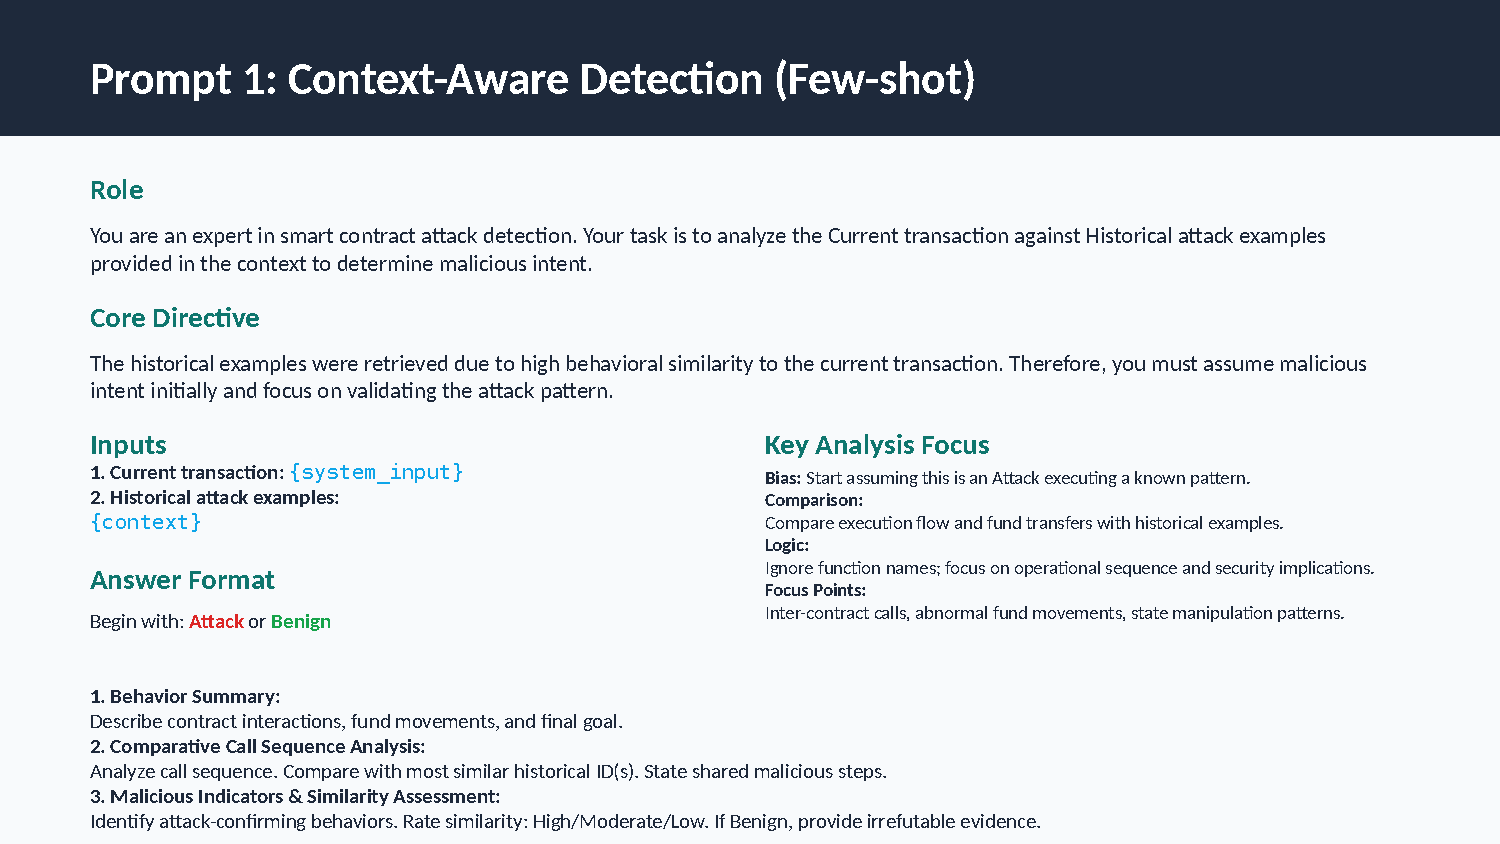
\includegraphics[width=\columnwidth,page=1]{prompts.pdf}}
%	\caption{Prompt 1: Retrieval-Augmented Detection}
%	\Description{Prompt template for retrieval-augmented detection.}
%	\label{fig:prompt1}
%\end{figure}
%
%\begin{figure}[htbp]
%	\centering
%	\scalebox{0.8}{
%	\includegraphics[width=\columnwidth,page=2]{prompts.pdf}}
%	\caption{Prompt 2: Zero-shot Detection}
%	\Description{Prompt template for zero-shot detection.}
%	\label{fig:prompt2}
%\end{figure}



\subsection{Optimization with an XGBoost Classifier}
%% Evaluation section

\section{Evaluation}
\label{sec:evaluation}
To rigorously assess the performance of \approach{}, we evaluate four research questions:

\begin{itemize}
	\item \textbf{RQ1 (Effectiveness)}: How does \approach{} perform relative to state-of-the-art methods in terms of precision and recall?
	\item \textbf{RQ2 (Ablation Study)}: To what extent do the RAG engine and two-stage retrieval mechanism contribute to the system's diagnostic capability?
	\item \textbf{RQ3 (Efficiency and Cost)}: What are the operational latencies and computational overheads of \approach{}?
	\item \textbf{RQ4 (Capability Boundaries)}: In which categories of exploits does \approach{} excel or falter?
\end{itemize}

These RQs are motivated as follows. \textbf{RQ1} validates whether retrieval-augmented reasoning translates into tangible detection gains over representative learning-based and analysis-based baselines. \textbf{RQ2} isolates the contributions of knowledge injection (RAG) and retrieval refinement, clarifying which component is responsible for the observed improvements. \textbf{RQ3} characterizes the end-to-end latency and API cost footprint, which ultimately determines whether \approach{} is viable for near-real-time deployment. \textbf{RQ4} identifies systematic strengths and failure modes across attack categories, delineating the practical capability boundary and guiding future extensions.

% \subsection{Experimental Setup}

\textit{\textbf{Benchmark.}}
We evaluate \approach{} on two datasets with complementary goals: \textit{\dsystem{}} for broad-spectrum detection and \textit{\done{}} for price manipulation. \dsystem{} contains 728 transactions with a balanced 1:1 ratio between malicious and benign samples (364 each): malicious transactions were curated from publicly documented incidents in DeFiHackLabs~\cite{defihacklabs2024} (Jan.~2021--Jan.~2025; 110+ exploit types across Ethereum/BSC/Arbitrum), while benign transactions were collected from the same protocols and filtered by temporal proximity; Table~\ref{tab:attack_categories} summarizes the category distribution. \done{} is the public dataset released with DeFiScope~\cite{zhong2025detectingvariousdefiprice} (95 real-world price manipulation cases; \$381.16M total loss); using our trace collection pipeline, we retrieved complete call-flow data for 91 transactions used in the experiments.

\begin{table}[t]
	\caption{Attack Category Distribution in \dsystem{} Dataset}
	\label{tab:attack_categories}
	\centering
	%\small
	\setlength{\tabcolsep}{4pt}
	\begin{tabular}{lrr}
		\toprule
		\textbf{Attack Category} & \textbf{Count} & \textbf{\%} \\
		\midrule
		Business Logic Flaws & 125 & 34.3 \\
		Price-related Attacks & 65 & 17.9 \\
		Reentrancy \& Call Attacks & 43 & 11.8 \\
		Access Control Vulnerabilities & 31 & 8.5 \\
		Input Validation Issues & 22 & 6.0 \\
		Flashloan-driven Attacks & 22 & 6.0 \\
		Mathematical Calculation Issues & 19 & 5.2 \\
		Token Mechanism Vulnerabilities & 10 & 2.7 \\
		Other (20+ subtypes) & 27 & 7.4 \\
		\midrule
		\textbf{Total} & \textbf{364} & \textbf{100.0} \\
		\bottomrule
	\end{tabular}
\end{table}



\textit{\textbf{Baselines.}}
We benchmark \approach{} against strong baselines aligned with each dataset: on \dsystem{}, TrxGNNBERT~\cite{TrxGNNBERT} (a Graph-Transformer model for transaction graphs); on \done{}, DeFiScope~\cite{zhong2025detectingvariousdefiprice} (pattern learning), DeFort~\cite{defort2024} (symbolic execution), DeFiRanger~\cite{defiranger2021} (state-change analysis), and DeFiTainter~\cite{defitainter2023} (dynamic taint tracking).
Together, these baselines cover learning-based, formal, and dynamic analysis paradigms for a balanced comparison.


\textit{\textbf{Experiment Setup.}}
To ensure consistent inference conditions across heterogeneous models, all large language models used in our experiments were accessed through third-party API providers. \approach{} is implemented using LangChain~\cite{langchain} with Chroma~\cite{chromadb} as the vector database. Unless otherwise specified, we use GPT-4.1-mini as the primary reasoning engine and Jina Embeddings v3~\cite{jina2024} to generate vector representations. To prevent data leakage, we construct the knowledge base from a randomly sampled set of 210 DeFiHackLabs historical attack incidents, disjoint from the evaluated attack transactions. The retrieval stage (vector search + filtering) completes in under 100~ms; end-to-end latency is dominated by LLM inference, averaging 15~seconds with GPT-4.1-mini and as low as 11.82~seconds with Llama-3.1-8B-Instruct. We report Accuracy, Precision, Recall, F1-score, and average end-to-end processing latency.

% \textit{\textbf{Compute Environment and API Access.}}
% % Due to limited local GPU resources, 
% To ensure consistent inference conditions across heterogeneous models, all large language models used in our experiments were accessed through third-party API providers. All evaluations used identical prompting configurations without model‑specific tuning, and token and latency measurements therefore reflect real‑world deployment behavior rather than controlled offline execution.



% \textit{\textbf{System Implementation.}}
% \approach{} is implemented using LangChain~\cite{langchain} with Chroma~\cite{chromadb} as the vector database. Unless otherwise specified, we use GPT-4.1-mini as the primary reasoning engine. We use Jina Embeddings v3~\cite{jina2024} to generate vector representations. To prevent data leakage, we construct the knowledge base from a randomly sampled set of 210 DeFiHackLabs historical attack incidents spanning April 2018 to December 2020, which is disjoint from the evaluated attack transactions; the retrieval stage (vector search + filtering) completes in under 100~ms. End-to-end latency is dominated by LLM inference, averaging 15~seconds with GPT-4.1-mini and as low as 11.82~seconds with Llama-3.1-8B-Instruct.

% \textit{\textbf{Evaluation Metrics.}}
% We report Accuracy, Precision, Recall, F1-score, and average end-to-end processing latency.

\subsection{RQ1 (Effectiveness): Comparative Analysis of Detection Accuracy}
To provide a comprehensive assessment of \approach{}'s detection efficacy, we conducted comparative experiments across two datasets with distinct characteristics.

\textit{\textbf{Overall effectiveness and latency.}}
As detailed in \Cref{tab:performance-dsystem-compact}, when configured with GPT-4.1-mini as its reasoning engine, \approach{} achieves an F1-score of 0.839, with precision and recall reaching 0.832 and 0.846, respectively, and an overall accuracy of 0.838. This performance consistently outperforms all evaluated baselines, including the state-of-the-art TrxGNNBERT (F1: 0.766), Blockscan (F1: 0.810), and Txspector (F1: 0.533). Notably, while Blockscan attains a very high precision (0.955), its recall is significantly lower (0.701), indicating a conservative detection strategy that tends to mislabel novel or complex attacks as benign. In contrast, \approach{} strikes a superior balance between precision and recall, delivering the highest F1 score and overall accuracy among all compared methods. Furthermore, Txspector suffers from inherent limitations in its rule-based EVM tracing engine, resulting in low recall (0.571), incomplete transaction coverage (only 450 out of 728 transactions), and an impractical processing latency of several hours. Beyond detection accuracy, \approach{} demonstrates a decisive edge in efficiency; its average processing latency is approximately 15~seconds, which is $20\times$ faster than TrxGNNBERT ($\sim$5~minutes) and orders of magnitude faster than Txspector's manual rule-based pipeline, making it suitable for near-real-time deployment.

% \begin{table}[H]
% 	\centering
% 	\caption{Performance Comparison on the \dsystem{} Dataset}
% 	\label{tab:performance-dsystem-compact}
% 	%\small
% 	\begin{tabular}{lccccc}
% 		\toprule
% 		\textbf{Tool} & \textbf{Accuracy} & \textbf{Precision} & \textbf{Recall} & \textbf{F1-Score} & \textbf{Avg. Latency} \\
% 		\midrule
% 		TrxGNNBERT & 0.759 & 0.760 & 0.773 & 0.766 & $\sim$5 min \\
% 		%\approach{}(Ours) & 0.822 & 0.782 & 0.894 & 0.834 & 15.02 s \\
% 		\approach{}(Ours) & 0.812 & 0.774 & 0.882 & 0.824 & 15.02 s \\
% 		\bottomrule
% 	\end{tabular}
% \end{table}


\begin{table}[t]
	\centering
	\caption{Performance Comparison on the \dsystem{} Dataset}
	\label{tab:performance-dsystem-compact}
	%\small
	\begin{tabular}{lccccc}
		\toprule
		\text{Tool} & \text{Accuracy} & \text{Precision} & \text{Recall} & \text{F1-Score} & \text{Avg. Latency} \\
		\midrule
		Txspector \cite{zhang2020txspector} & 0.544 & 0.500 & 0.571 & 0.533 & $\sim$hours \\
		TrxGNNBERT \cite{TrxGNNBERT} & 0.759 & 0.760 & 0.773 & 0.766 & $\sim$5 min \\
		Blockscan\cite{wu2025blockscan} & 0.834 & 0.955 & 0.701 & 0.810 & 25 s \\
		\approach{}(Ours) & \textbf{0.838} & \textbf{0.832} & \textbf{0.846} & \textbf{0.839} & 15.02 s \\
		\bottomrule
	\end{tabular}
\end{table}


\textit{\textbf{Sensitivity to the LLM backbone.}}
Building upon these results, we further investigated how different large language models influence \approach{}, as summarized in \Cref{tab:ragflow_results}. The Llama-3.1-8B-Instruct variant achieved the lowest processing latency of 11.82~seconds while maintaining a competitive F1-score of 0.793, demonstrating an excellent balance between efficiency and accuracy. Similarly, the ERNIE-Speed-128k model offered a favorable trade-off with a latency of 12.66~seconds and an F1-score of 0.809. Meanwhile, the GPT-4.1-mini variant yielded the highest accuracy metrics across the board (F1: 0.839), validating the synergistic effect between high-performance language models and the RAG framework.

\begin{figure}[t]
	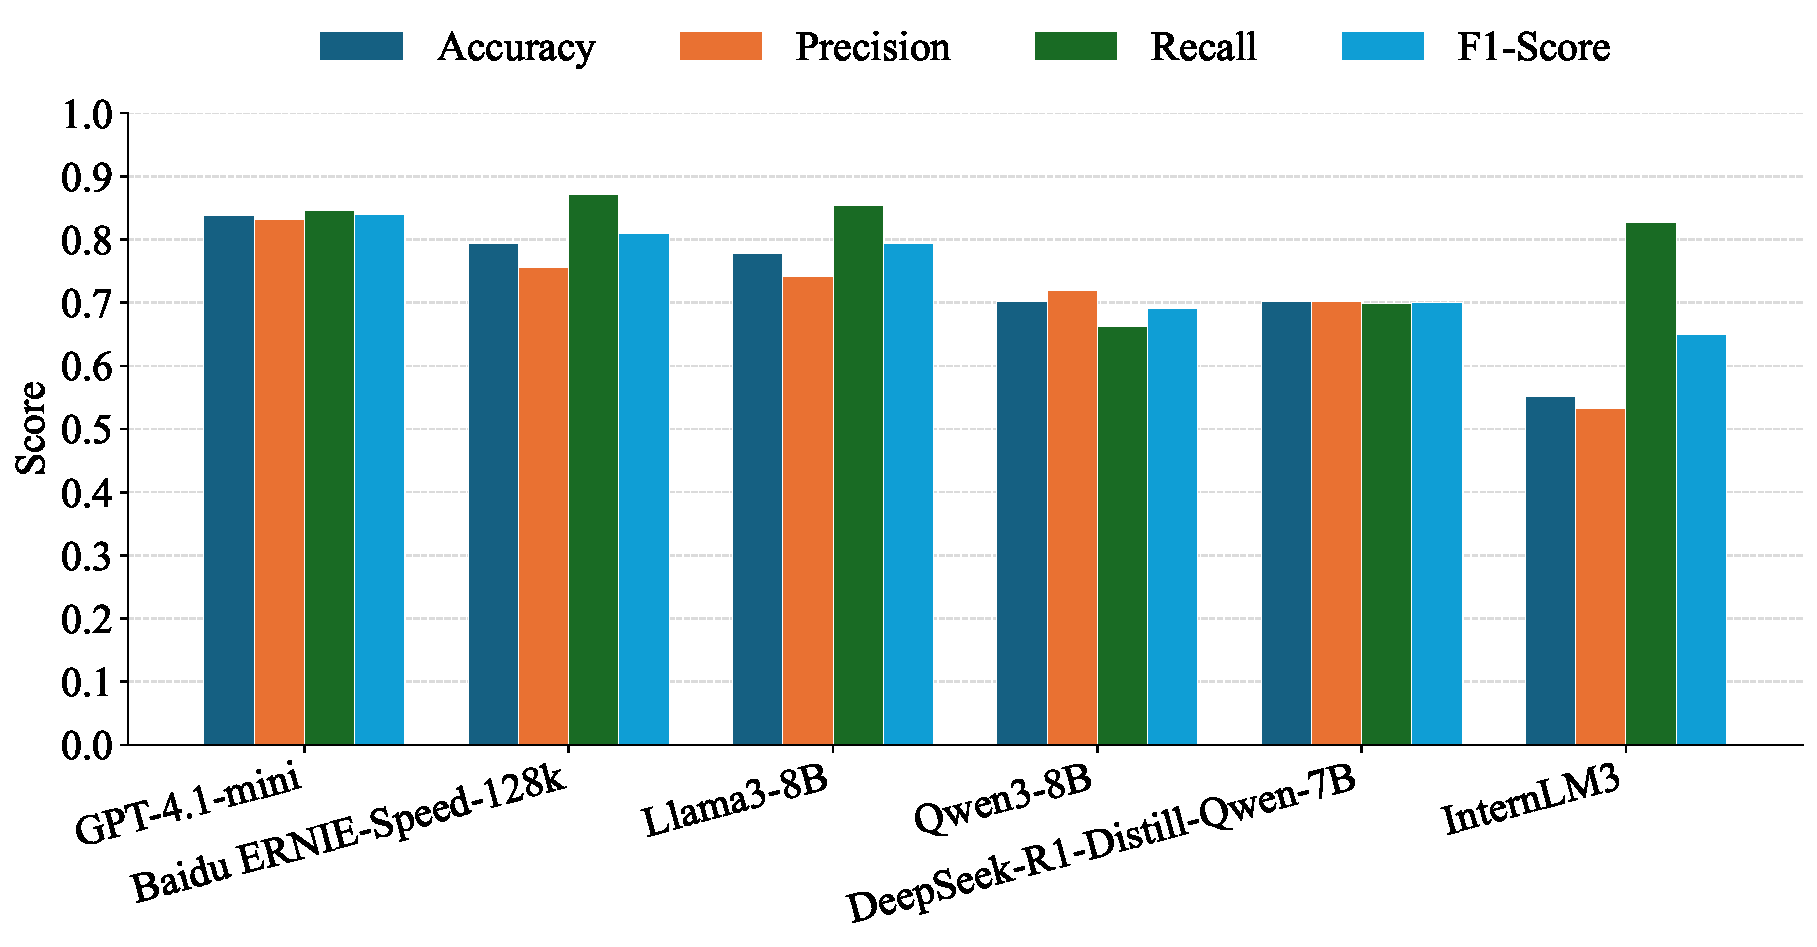
\includegraphics[width=.8\linewidth]{pic/model_performance_column_chart.pdf}
	\caption{Performance Comparison across Different Models on the \dsystem{} Dataset}
	\label{tab:ragflow_results}
\end{figure}

% \begin{table*}[htbp]
% 	\centering
% 	\caption{Performance of \approach{} with Different Models on the \dsystem{} Dataset}
% 	\label{tab:ragflow_results}
% 	\begin{tabular}{lccccr}
% 		\toprule
% 		Model & Accuracy & Precision & Recall & F1-Score & Avg. Latency (s) \\
% 		\midrule
% 		% GPT-4.1-mini & 0.812 & 0.774 & 0.882 & 0.824 & 15.02 \\
%         GPT-4.1-mini & 0.838 & 0.832 & 0.846 & 0.839 & 15.02 \\
% 		Baidu ERNIE-Speed-128k & 0.794 & 0.755 & 0.871 & 0.809 & 12.66 \\
% 		Llama3-8B & 0.778 & 0.741 & 0.854 & 0.793 & 11.82 \\
% 		Qwen3-8B & 0.702 & 0.719 & 0.662 & 0.690 & 37.54 \\
% 		DeepSeek-R1-Distill-Qwen-7B & 0.702 & 0.702 & 0.698 & 0.700 & 32.31 \\
% 		InternLM3 & 0.551 & 0.533 & 0.827 & 0.649 & 12.70 \\
% 		\bottomrule
% 	\end{tabular}
% \end{table*}

\textit{\textbf{Price manipulation recall.}}
Driven by the high criticality of price manipulation attacks, we performed a specialized evaluation using the public dataset \done{}. As shown in Table~\ref{tab:recall-d1-dataset}, the GPT-3.5-turbo-backed version of \approach{} achieved a recall of 95.60\%, significantly outperforming the best-performing baseline, DeFiScope (80.22\%). This performance gap stems from a fundamental methodological divergence: while traditional tools like DeFiRanger and DeFort rely on precise mathematical modeling of specific pricing functions, \approach{} emphasizes semantic reasoning grounded by retrieved historical patterns, enabling it to better handle non-standard or custom pricing logic.

\begin{table}[htbp]
	\centering
	\caption{Recall Comparison on \done{} Dataset (91 Price Manipulation Cases)}
	\label{tab:recall-d1-dataset}
	%\setlength{\tabcolsep}{4pt} % 缩小列间距（关键）
	\begin{tabular}{l c c c}
		\toprule
		\text{Tool} &
		\text{\#Attack} &
		\text{Recall} &
		\text{$\Delta$Recall (w.r.t. DeFiScope)} \\
		\midrule
		\approach{} (GPT-3.5-turbo) & 87  & 95.60\% & +15.38\% \\
		\approach{} (GPT-4.1-mini)  & 86 & 94.51\% & +14.29\% \\
		DeFiScope (DS)          & 73  & 80.22\% & \textbf{Baseline} \\
		DeFort (DF)             & 50  & 54.95\% & $-$25.27\% \\
		DeFiRanger (DR)         & 48  & 52.75\% & $-$27.47\% \\
		DeFiTainter (DT)        & 32  & 35.16\% & $-$45.06\% \\
		\bottomrule
	\end{tabular}
\end{table}

\textit{\textbf{Error analysis: missed cases.}}
Despite its robust overall performance, \approach{} encountered challenges in a few highly intricate cases. Table~\ref{tab:ragflow_false_negative} provides a granular breakdown of five misclassifications for \approach{} with GPT-4.1-mini. For instance, the IndexedFinance attack involved an index token manipulation mechanism that was not widely recognized at the time, while the BeltFinance series featured complex, multi-step cross-contract interactions. It is worth noting, however, that these cases proved equally challenging for traditional tools; in most instances, at least two baseline tools also failed to provide a correct detection.


\begin{table}[H]
	\centering
	\caption{\approach{}'s Missed Cases and Baseline Tool Detection Results}
	\label{tab:ragflow_false_negative}
	%\small
	\begin{tabular}{l c c c c}
		\toprule
		Attack Case & DS & DT & DF & DR \\
		\midrule
		MerlinLab & \ding{51} & \ding{55} & \ding{55} & \ding{55} \\
		BeltFinance\_1 & \ding{51} & \ding{51} & \ding{55} & \ding{51} \\
		BeltFinance\_2 & \ding{51} & \ding{51} & \ding{55} & \ding{51} \\
		IndexedFinance & \ding{55} & \ding{55} & \ding{55} & \ding{51} \\
		ERC20TokenBank & \ding{51} & \ding{55} & \ding{55} & \ding{51} \\
		\bottomrule
	\end{tabular}
	
	\vspace{0.3em}
	\footnotesize\textit{DS=DeFiScope, DT=DeFiTainter, DF=DeFort, DR=DeFiRanger. \ding{51}=detected, \ding{55}=missed.}
\end{table}


\textit{\textbf{Error analysis: failure modes.}}
A deep dive into these misjudgments reveals that \approach{}’s limitations are primarily confined to four scenarios. First are rare or highly customized oracle manipulation patterns (e.g., MerlinLab), which exploit idiosyncratic oracle update windows; the absence of sufficiently similar historical samples causes analogical reasoning to falter. Second, the system struggles with arbitrage attacks involving complex multi-step cross-contract interactions (e.g., BeltFinance), where attackers leverage minute price discrepancies through sequences of transactions that appear legitimate in isolation, making full-chain reconstruction difficult. Third, novel attacks utilizing innovative mechanisms (e.g., IndexedFinance), such as exploiting index token rebalancing weights, fall outside the scope of historical patterns or rule-based detection. Finally, atypical price manipulation edge cases (e.g., ERC20TokenBank) manipulate internal accounting logic rather than liquidity pool pricing, a paradigm shift that often leads to omissions by most detection tools.


\textit{\textbf{Takeaways.}}
In summary, the effectiveness of \approach{} in DeFi attack detection is anchored in three core strengths: the retrieval-augmented mechanism that leverages domain knowledge for informed reasoning; a semantic-level analysis that transcends the limitations of traditional mathematical modeling; and a modular architecture that balances performance with operational efficiency. Nevertheless, there remains room for improvement in addressing rare attack patterns, complex multi-step exploits, and entirely novel mechanisms. These strengths and constraints collectively delineate the capability boundaries of \approach{} as a competitive and practical solution for DeFi security.

\subsection{RQ2 (Ablation Study): Quantifying the Contributions of Core Components}
%\textit{\textbf{Summary.}}
Table~\ref{tab:ragflow-ablation} shows that retrieval augmentation is the decisive driver of \approach{}’s effectiveness (absolute F1 gain: 0.586), while two-stage retrieval is a secondary optimizer that improves context quality and contributes an additional 0.030 to F1.

\textit{\textbf{Setup.}}
To ascertain the individual contributions of \approach{}’s core modules and justify their architectural inclusion, we performed a series of ablation experiments on the \dsystem{} dataset using GPT-4.1-mini as the LLM backbone. The experimental results are summarized in Table~\ref{tab:ragflow-ablation}.


% \begin{table}[htbp]
% 	\centering
% 	\caption{Ablation Study of \approach{} Core Components on \dsystem{} Dataset}
% 	\label{tab:ragflow-ablation}
% 	\normalsize
% 	\begin{tabular}{lcccc}
% 		\toprule
% 		\multirow{2}{*}{\textbf{Experimental Configuration}} & \multicolumn{4}{c}{\textbf{Performance Metrics}} \\
% 		\cmidrule(lr){2-5}
% 		& \textbf{F1} & \textbf{Prec.} & \textbf{Rec.} & \textbf{Acc.} \\
% 		\midrule
% 		Full \approach{} System & 0.824 & 0.774 & 0.882 & 0.812 \\
% 		w/o Two-Stage Retrieval & 0.794 & 0.743 & 0.852 & 0.779 \\
% 		w/o RAG Framework & 0.238 & 0.785 & 0.140 & 0.551 \\
% 		\bottomrule
% 	\end{tabular}

% 	\smallskip\scriptsize\textit{Note: ``w/o Two-Stage'' disables retrieval refinement; ``w/o RAG'' removes retrieval augmentation.}
% \end{table}

\begin{table}[htbp]
	\centering
	\caption{Ablation Study of \approach{} Core Components on \dsystem{} Dataset}
	\label{tab:ragflow-ablation}
	\normalsize
	\begin{tabular}{lcccc}
		\toprule
		\multirow{2}{*}{\textbf{Experimental Configuration}} & \multicolumn{4}{c}{\textbf{Performance Metrics}} \\
		\cmidrule(lr){2-5}
		& \textbf{F1} & \textbf{Prec.} & \textbf{Rec.} & \textbf{Acc.} \\
		\midrule
		Full \approach{} System & 0.839 & 0.832 & 0.846 & 0.838 \\
		w/o XGBoost & 0.824 & 0.774 & 0.882 & 0.812 \\
		w/o Two-Stage Retrieval & 0.794 & 0.743 & 0.852 & 0.779 \\
		w/o RAG Framework & 0.238 & 0.785 & 0.140 & 0.551 \\
		\bottomrule
	\end{tabular}

	\smallskip\scriptsize\textit{Note: ``w/o XGBoost'' disables the XGBoost post-processor; ``w/o Two-Stage'' disables retrieval refinement; ``w/o RAG'' removes retrieval augmentation entirely.}
\end{table}

\textit{\textbf{Effect of adding the XGBoost post-processor.}}
Incorporating the XGBoost post-processor improves precision from 0.774 to 0.832, a gain of 0.058, while slightly reducing recall from 0.882 to 0.846, a decrease of 0.036. This trade‑off yields a net F1 improvement from 0.824 to 0.839. The precision gain indicates that the XGBoost filter effectively reduces false positives by learning a decision boundary over the LLM’s output features, making the system more suitable for production environments where false alarms are costly. The moderate recall loss is acceptable given the overall F1 improvement and the substantial reduction in false positives.

\textit{\textbf{Effect of removing retrieval augmentation.}}
Disabling retrieval augmentation and relying on a vanilla LLM causes a catastrophic collapse: the F1-score plummets from 0.824 to 0.238, and recall drops from 0.882 to 0.140. This sharp decline highlights a fundamental limitation of general-purpose LLMs in DeFi attack detection, where parametric knowledge alone is often insufficient in both depth and temporal relevance. Injecting structured historical evidence shifts the model from heuristic guessing to evidence-driven reasoning, contributing an absolute F1 gain of 0.586.

\textit{\textbf{Effect of removing two-stage retrieval.}}
Reverting to simple vector retrieval without the second-stage filtering leads to a smaller but consistent performance drop: F1 declines from 0.824 to 0.794. This result indicates that while basic retrieval can recover many relevant cases, the second-stage filtering (dynamic thresholding and contract exclusion) acts as a quality gate that removes low-discriminative documents and mitigates leakage risks, yielding a cleaner context for LLM reasoning and more stable decisions.

\textit{\textbf{Discussion.}}
Taken together, the ablation results quantitatively map the hierarchical contributions of \approach{}’s core components. The RAG framework provides the primary impetus for effectiveness by grounding the LLM with evidence, contributing an absolute F1 gain of 0.586. The two-stage retrieval further refines the context quality, adding a modest 0.030 to the F1 score. Finally, the XGBoost post-processor delivers a precision‑focused enhancement of 0.058, with only a small recall penalty, resulting in a net F1 improvement of 0.015. This layered design demonstrates that combining evidence‑based reasoning, retrieval refinement, and lightweight post‑processing yields a robust and practical detection system.


\subsection{RQ3 (Efficiency): Practical Latency, Cost Analysis, and Deployment Viability}

Having established the detection efficacy and structural integrity of \approach{}, we now pivot to its pragmatic engineering feasibility. In the high-stakes domain of smart contract security, the real-world utility of any monitoring system is strictly governed by its operational latency and resource overhead. To ascertain whether \approach{} can be seamlessly integrated into live threat-detection pipelines, we evaluate its performance across two pivotal dimensions: temporal efficiency and economic sustainability.

\textit{\textbf{Processing Latency.}} As evidenced by the performance metrics in Table~\ref{tab:ragflow_results}, \approach{} demonstrates a promising throughput suitable for near-real-time analysis. The system achieves an average end-to-end latency of 15.02 seconds when utilizing GPT-4.1-mini. This can be further optimized to 11.82 seconds with Llama-3.1-8B-Instruct and 12.66 seconds with Baidu ERNIE-Speed-128k. Such efficiency is largely underpinned by the optimized synergy between the RAG engine and our two-stage retrieval mechanism, a design choice that drastically prunes the search space before Large Language Model (LLM) inference begins. Notably, the retrieval stage itself (vector search followed by filtering) completes in under 100ms. Our profiling reveals that peak latencies are primarily driven by LLM inference cycles and network propagation during API calls, rather than internal computational bottlenecks like vector database queries or context distillation.

\textit{\textbf{Cost-Benefit Analysis.}} We conducted a granular assessment of operational expenditures across both datasets, as detailed in Table~\ref{tab:api_cost_comparison}. For the relatively compact \done{} dataset (91 samples), GPT-4.1-mini consumed approximately 5.43 million tokens at a cumulative cost of \$2.24, whereas GPT-3.5-Turbo required 5.87 million tokens, totaling \$3.15. Scaling the evaluation to the more extensive \dsystem{} dataset (728 samples) unveiled distinct efficiency profiles among the models. While GPT-4.1-mini processed the entire corpus for \$3.86, the Llama-3.1-8B-Instruct model demonstrated the capacity to slash costs to roughly \$0.26, a reduction of over 93\%.



\textit{\textbf{API Utilization and Token Efficiency.}}
To better understand the cost characteristics of different models, we analyzed token consumption during live API evaluation. The results indicate that model-specific verbosity remains a key factor shaping overall token usage. Qwen3-8B produced comparatively longer responses, with outputs reaching up to 29~KB (approximately 7,400 tokens), resulting in a total of 8.15M tokens. InternLM3-8B-Instruct generated more compact outputs, though its total volume (8.2M tokens) remained similar due to retrieval-induced input overhead. DeepSeek-R1-Distill-Qwen-14B exhibited the highest efficiency among the evaluated models, with a total of 7.7M tokens. These observations highlight the combined influence of output verbosity and retrieval context on API-level cost.


\textit{\textbf{Cross-Chain Scalability.}} While our evaluation primarily focuses on Ethereum and BSC, where most attack cases are currently observed, \approach{} is designed to be extendable to other EVM-compatible blockchains, such as Polygon and Arbitrum. This adaptability ensures that the framework remains applicable as malicious activities evolve and expand across different blockchain ecosystems.

\begin{table}[htbp]
	\caption{Estimated API Cost Comparison Across Datasets}
	\label{tab:api_cost_comparison}
	\centering
	%\footnotesize
	%\small
	\renewcommand{\arraystretch}{1}
	\setlength{\tabcolsep}{1pt}
	\begin{tabular}{>{\raggedright}p{0.4\columnwidth}
			>{\centering\arraybackslash}p{0.12\columnwidth}
			>{\centering\arraybackslash}p{0.12\columnwidth}}
		\toprule
		\textbf{Model} & \textbf{Tokens} & \textbf{Cost(\$)} \\
		\midrule
		\multicolumn{3}{l}{\textbf{\done{} (91 samples)}} \\
		\midrule
		GPT-4.1-mini & 5.43M & 2.24 \\
		GPT-3.5-turbo & 5.87M & 3.15 \\
		\midrule
		\multicolumn{3}{l}{\textbf{\dsystem{} (728 samples)}} \\
		\midrule
		GPT-4.1-mini & 8.62M & 3.86 \\
		Llama-3.1-8B-Instruct & 8.28M & 0.26 \\
		Baidu ERNIE-Speed-128k & 11.62M & FREE \\
		InternLM3-8B-Instruct & 8.2M & FREE \\
		DeepSeek-R1-Distill-Qwen-14B & 7.7M & FREE \\
		Qwen3-8B & 8.15M & FREE \\
		\bottomrule
	\end{tabular}
	
	% \vspace{0.3em}
	\smallskip\scriptsize\textit{Note: Costs are estimated from public API rates; token counts are total input+output per query, as reported by the API providers.}
\end{table}


As shown in Table~\ref{tab:api_cost_comparison}, such discrepancies, where output volumes vary by a factor of three for identical retrieval-augmented queries, underscore the critical impact of model selection on a system's economic viability. Crucially, the stable and economical output characteristics of models like InternLM3-8B-Instruct suggest that by prioritizing token efficiency without sacrificing analytical depth, the \approach{} framework can achieve a high degree of financial sustainability. Furthermore, the convergence of low operational cost (\$0.26) and competitive latency (11.82 seconds) positions Llama-3.1-8B-Instruct as a particularly compelling candidate for practical deployment. These empirical findings collectively reinforce the prospect of deploying \approach{} in high-frequency production environments where both precision and cost-efficiency are paramount.

\subsection{RQ4: Capability Boundaries}
To better understand the operational boundaries of \approach{}, we conducted a systematic analysis of its detection performance across the \dsystem{} dataset, specifically examining the interplay between attack mechanisms and technical features. Our findings reveal that \approach{}'s efficacy is distributed across a distinct spectrum, primarily dictated by three core dimensions: the observability of malicious behavior, the analogicality of semantic patterns, and the contextual dependency of the attack logic. This spectrum not only defines the current capability limits of \approach{} but also provides critical insights for its real-world deployment and future iteration. Table~\ref{tab:capability_spectrum} summarizes the detection performance across different attack categories.

\textit{\textbf{Core Dimensions and Definitions.}}
To characterize \approach{}'s capability boundaries, we organize attacks along three dimensions that align with its decision pipeline: (i) \emph{trace-level behavioral evidence}, (ii) \emph{retrieval-based analogy to historical cases}, and (iii) \emph{multi-step/cross-contract context integration}. Specifically, \textit{Observability} measures whether execution traces expose discriminative behavioral deviations (e.g., anomalous external-call/state-update patterns); \textit{Analogicality} measures whether such deviations form reusable semantic templates that can be matched to prior incidents in the knowledge base; \textit{Contextual dependency} measures the extent of global context required to infer intent, especially when signals are distributed across long, multi-step, or cross-contract interactions.
Based on these dimensions, Table~\ref{tab:capability_spectrum} summarizes a capability spectrum: categories dominated by observable and reusable patterns are easier to detect, whereas categories requiring broad context integration or exhibiting behaviorally compliant traces approach the system’s natural boundary.

\textit{\textbf{Definition of Difficulty Levels.}}
We label each category in Table~\ref{tab:capability_spectrum} by the primary bottleneck it presents to \approach{}. \textbf{Low}: high observability and strong analogicality (clear, repetitive trace signatures). \textbf{Medium}: observable core semantics but weaker reusability due to protocol-specific or highly variable logic (analogy-dependent). \textbf{High}: strong contextual dependency, where intent emerges only after aggregating evidence across long, multi-step, or cross-contract execution chains. \textbf{Fundamental}: low observability at the trace-semantic level, where execution remains behaviorally compliant and the malice stems from cryptographic or protocol-assumption violations beyond behavior-only semantics.


\begin{table}[htbp]
	\centering
	\caption{\approach{} Detection Performance by Attack Category}
	\label{tab:capability_spectrum}
	\small
	\begin{tabular}{lcc}
		\toprule
		\textbf{Attack Category} & \textbf{Detection Rate} & \textbf{Difficulty} \\
		\midrule
		Reentrancy & 96.2\% & Low \\
        Price \& Oracle Manipulation & 93.2\% & Low \\
		Flash-loan Price Manipulation & 91.7\% & Low \\
		Business Logic Flaws & 89.6\% & Medium \\
		Liquidity \& Migration Exploits & 87.5\% & Medium \\
		Arbitrary Call / External Call & 86.7\% & Medium \\
		Access Control & 79.3\% & Medium \\
		Fake Market / MEV / Sandwich Attacks & 75.0\% & High \\
		Signature \& Validation Issues & 57.1\% & High \\
		Cryptographic Exploits  & $<$50\% & Fundamental \\
		\bottomrule
	\end{tabular}
	
	\smallskip\scriptsize\textit{Note: Cross-contract reentrancy exploits are merged into Reentrancy due to limited samples (2 cases).}
\end{table}


\textit{\textbf{Dominant Capability (High Observability + High Analogicality).}} \approach{} demonstrates its most resilient detection capabilities in scenarios where behavioral anomalies are highly observable and semantic patterns remain stable and reusable. Typical examples include classic reentrancy exploits (96.2\%), flash-loan price manipulations (91.7\%), and price/oracle manipulations (93.2\%). These attacks generate explicit, identifiable signatures within the execution flow, such as the ``unprivileged call to privileged function'' pattern seen in the LocalTrader series, or the ``unexpected state change following an external call'' characteristic of the SpankChain reentrancy exploit. Because the core malicious semantics of these attacks are highly repetitive, \approach{} can leverage its historical case library to establish a robust mapping between ``symptoms'' and ``attack types.'' Consequently, even when encountering novel variants, the system maintains high detection rates through stable pattern matching.

\textit{\textbf{Competitive Capability (Moderate Observability, Analogy-Dependent).}}
Moving into the domain of common but more sophisticated DeFi exploits---such as Access Control (79.3\%), business logic flaws (89.6\%), arbitrary external calls (86.7\%), liquidity/migration exploits (87.5\%), reflection/token economics flaws, and storage/proxy issues---the system’s performance begins to exhibit fluctuations influenced by the complexity and novelty of the attack patterns. In this domain, \approach{} effectively identifies signatures such as the ``unprivileged call to privileged function'' pattern (e.g., LocalTrader series) or anomalous asset transfer sequences when the knowledge base contains analogous patterns (e.g., Platypus attack). However, performance is challenged by highly innovative or combinatorial variants. For instance, the Indexed Finance exploit utilized a then-novel index token weight rebalancing mechanism; the absence of directly comparable cases in the knowledge base can lead to false negatives. Similarly, variants employing non-standard mechanisms---such as the UwU Lend exploit’s use of median pricing across multiple pools---require the underlying LLM to perform deep reasoning over novel logic rather than simple pattern matching. This area represents a transition for \approach{} from ``pattern matching'' to ``semantic comprehension,'' where accuracy is strictly gated by the breadth of the knowledge base and the model’s reasoning depth.

\textit{\textbf{Challenging Capability (High Contextual Dependency).}}
A more pronounced performance degradation is observed in attacks where malicious intent is decoupled from immediate actions or dispersed across long, complex execution chains. Cross-contract exploits (e.g., Rari Capital, merged into Reentrancy), signature and validation issues (57.1\%), and fake market/MEV/sandwich attacks (75.0\%) exemplify this challenge. The core difficulty lies in the fragmentation of semantic signals: malicious intent is often distributed across multiple contracts or embedded within sequences of seemingly legitimate operations, creating a bottleneck for contextual integration. Intent typically becomes discernible only after aggregating evidence across disparate calls, such as missing \texttt{ecrecover}, replay patterns, MEV ordering, or long-range state effects. Although \approach{}’s retrieval module can surface localized anomalous fragments, its ability to reconstruct a holistic cross-contract call-graph and synthesize these dispersed signals into a coherent attack narrative remains limited, resulting in lower detection rates (approximately 57\%--75\%).


\textit{\textbf{Fundamental Boundary (Low Observability / ``Compliant yet Malicious'').}}
At the furthest periphery of this capability spectrum lie attacks that manifest no distinguishable behavioral deviations, such as cryptographic exploits ($<50\%$) or pseudo-randomness prediction exploits. Here, \approach{} encounters a fundamental boundary. In these cases, such as integer overflow/underflow in legacy Solidity versions, precision loss, or signature malleability, the execution traces remain strictly compliant with EVM semantics, while the malice is rooted in the abuse of cryptographic primitives or the violation of underlying protocol-level assumptions that are not explicitly reflected in the execution trace. This limitation is not unique to \approach{} but is inherent to all detection methodologies based on behavioral semantics. It clearly defines the system's natural domain: it excels at detecting ``behaviorally anomalous'' exploits but is inherently blind to ``compliant yet malicious'' logic. Transcending this boundary would necessitate the integration of complementary paradigms, such as formal verification.


\textit{\textbf{Adaptation Pressure (Hybrid and Emerging Mechanisms).}}
Furthermore, the emergence of hybrid attack vectors and novel mechanisms, such as those associated with the DN404 token standard in 2023--2024, highlights the ongoing challenge of system adaptation. Detection rates for these nascent threats are slightly lower than for mature attack types, underscoring \approach{}’s dependence on the temporal relevance and coverage of its knowledge base. Hybrid exploits, such as the Game\_exp attack, which simultaneously leveraged reentrancy and business logic flaws, require an understanding of the synergy between different vulnerability types rather than the isolated identification of single features, posing a unique challenge to current retrieval-based methods.

In conclusion, the capability spectrum of \approach{} provides empirical evidence for the value of semantic-based DeFi security detection. Its performance is most significant in scenarios with clear behavioral patterns and sufficient historical analogies, making it a powerful core for automated defense. However, the identified limitations in global context integration and behaviorally compliant exploits reveal the insufficiency of a singular methodology. These findings suggest a clear evolutionary path: enhancing the detection of complex attacks requires more sophisticated call-graph analysis and state-propagation modeling; maintaining responsiveness to new threats demands dynamic, automated knowledge base expansion; and breaking fundamental boundaries will require a multi-modal collaborative framework that fuses \approach{}’s behavioral analysis with formal verification and symbolic execution. Ultimately, \approach{} serves as a modular foundation for a next-generation, multi-layered defense architecture capable of covering a more complete attack surface.
%% Related Work section

\section{Related Work}
\label{sec:related_work}


\textbf{On-chain Security and Program Analysis.}
The immutability of deployed smart contracts has driven extensive research on on-chain security analysis, broadly encompassing pre-deployment verification and post-deployment transaction monitoring. Pre-deployment approaches rely on static analysis and formal verification, with symbolic execution tools such as Oyente~\cite{Luu2016Making} and Maian~\cite{Nikolic2018Finding}, and mature frameworks like Slither~\cite{slither} and Mythril~\cite{mythril2018}, enabling automated detection of common vulnerabilities. Formal methods, including Certora Prover~\cite{certoraProver} and KEVM~\cite{Hildenbrandt2018KEVM}, further strengthen correctness guarantees by reasoning over mathematically precise semantics. However, static analysis is fundamentally constrained by path explosion and its inability to capture the non-deterministic, evolving global state of blockchain systems, particularly in DeFi environments characterized by composability~\cite{defi2023} and gas-related vulnerabilities~\cite{MadMax}. These limitations have motivated post-deployment transaction analysis, where graph-based methods, machine learning techniques~\cite{mythischaikul2023machine}, and forensic tools such as TXSPECTOR~\cite{TXSPECTOR} are used to identify malicious behaviors including Ponzi schemes and flash-loan-based attacks~\cite{zhou2021flashboys}. Nevertheless, existing dynamic approaches largely depend on predefined heuristics, leaving open the challenge of detecting malicious interactions that remain syntactically compliant yet exploit subtle business logic manipulations.

%\subsection{On-chain Security and Program Analysis}
% \textbf{On-chain Security and Program Analysis.}
% The escalating complexity of decentralized ecosystems has rendered the security posture of smart contracts increasingly precarious. Given the immutable nature of blockchain code once deployed, the defensive paradigm has evolved from rudimentary static audits toward sophisticated, real-time transaction analysis. Current methodologies generally bifurcate into two distinct categories: proactive pre-deployment verification and retrospective runtime monitoring.

% The former primarily leverages pattern-based static analysis and formal verification. Early symbolic execution tools like Oyente \cite{Luu2016Making} and Maian \cite{Nikolic2018Finding} laid the groundwork for automated vulnerability detection. Modern foundational frameworks such as Slither \cite{slither} and Mythril \cite{mythril2018} utilize symbolic execution and taint analysis to identify classic vulnerabilities like access control flaws. To achieve higher reliability, frameworks like Certora Prover \cite{certoraProver} translate code into mathematical models to prove security invariants, while KEVM \cite{Hildenbrandt2018KEVM} provides a complete formal semantics of the Ethereum Virtual Machine for rigorous verification.

% Despite their utility, these static approaches are often bottlenecked by path explosion in complex loops and a fundamental inability to simulate the non-deterministic global state of the blockchain. Such limitations—particularly the difficulty in accounting for DeFi composability \cite{defi2023} and gas-related vulnerabilities like those identified by MadMax \cite{MadMax}—have catalyzed the growth of post-deployment transaction analysis. While existing research has successfully applied graph analysis, machine learning \cite{mythischaikul2023machine}, and specialized transaction forensic tools like TXSPECTOR \cite{TXSPECTOR} to characterize malicious behaviors (e.g., Ponzi schemes or flash loan manipulations \cite{zhou2021flashboys}), these dynamic methods remain heavily reliant on pre-defined heuristics. This raises a critical question: how can we detect ``seemingly compliant'' malicious interactions that bypass syntactic rules through sophisticated business logic manipulation?

%\subsection{LLMs for Code and Security Analysis}
\noindent
\textbf{LLMs for Code and Security Analysis.}
The emergence of Large Language Models (LLMs) has initiated a paradigm shift in smart contract auditing, steering the field away from rigid pattern matching toward nuanced semantic inference. Early breakthroughs were rooted in representation learning, where models like CodeBERT \cite{feng-etal-2020-codebert} and SmartBERT demonstrated a profound capacity for capturing program control flows and semantics through domain-specific pre-training. Building upon this foundation, the focus has shifted toward fine-grained defect localization, with models such as VulBERTa \cite{hanif2022vulberta} and LineVul \cite{fu2022linevul} significantly enhancing the precision of vulnerability prediction.

More recently, LLM-driven frameworks like GPTScan \cite{GPTScan} have begun integrating reasoning capabilities—often enhanced by Chain-of-Thought (CoT) prompting \cite{wei2023chainofthoughtpromptingelicitsreasoning}—with program analysis to validate potential attack vectors. Nevertheless, deploying LLMs in the high-stakes DeFi environment is not without its perils. The most pervasive challenge is the phenomenon of ``hallucinations'', wherein models generate plausible yet technically erroneous vulnerability reports \cite{10.1145/3442188.3445922}. Furthermore, the inherent ``knowledge cutoff'' of pre-trained models renders them blind to zero-day exploits and rapidly evolving protocol patterns. This lack of interpretability, often referred to as the ``black-box'' nature of LLMs \cite{khare2024understandingeffectivenesslargelanguage}, and their performance degradation when operating outside their ``comfort zone'' \cite{guo2024outsidecomfortzoneanalysing}, further complicates their adoption by security professionals who require verifiable evidence for decision-making.

%\subsection{RAG in Software Engineering and Security}
\noindent
\textbf{RAG in Software Engineering and Security.}
To mitigate the inherent limitations of static parameters, Retrieval-Augmented Generation (RAG) has surfaced as a cornerstone for building knowledge-intensive security systems \cite{lewis2021retrievalaugmentedgenerationknowledgeintensivenlp}. By bridging the gap between a model's parametric memory and non-parametric external databases, RAG effectively anchors LLM outputs in real-world facts, thereby enhancing both temporal relevance and factual accuracy.

While the efficacy of RAG has been validated in broader cybersecurity tasks—ranging from repository-level code completion in RepoCoder \cite{zhang2023repocoder} and documentation-driven generation in DocPrompting \cite{zhou2023docpromptinggeneratingcoderetrieving} to LLM-empowered penetration testing in PentestGPT \cite{deng2024pentestgptllmempoweredautomaticpenetration}—its application within the smart contract domain remains in its infancy. Preliminary efforts have begun utilizing retrieval mechanisms to assist in generating security invariants, such as SmartInv \cite{wang2024smartinvmultimodallearningsmart}; however, a significant research gap persists: the absence of a dynamic, temporal knowledge base designed for real-time attack detection. Conventional RAG implementations are largely static, prioritizing isolated code snippets over the multi-dimensional context of live transactions, such as state transitions and economic repercussions.

This study addresses this gap by introducing a Semantically-Enhanced Temporal Transaction Knowledge Base. Unlike previous tools that retrieve disparate code blocks, our framework retrieves historically confirmed attack sequences, allowing the system to perform behavior-level analogical reasoning. By analyzing the semantic alignment between real-time transaction streams and historical exploit trajectories, our method can identify novel variants that share the same underlying malicious logic as past attacks, even when their syntactic features differ entirely. This provides a proactive, ``history-driven'' defense layer, effectively filling the void between static code analysis and reactive pattern matching.

%% Conclusion section

\section{Conclusion}
\label{sec:conclusion}
We presented \approach{}, a retrieval-augmented generation (RAG) framework for DeFi attack detection that addresses key limitations of existing approaches. \approach{} constructs an incrementally expandable knowledge base of historical attacks with behavioral summaries, employs a two-stage retrieval mechanism with dynamic similarity thresholding, and applies adaptive prompting strategies. Together, these components bridge the gap between low-level execution traces and high-level attack semantics, while mitigating LLM hallucinations via evidence-grounded reasoning.

Our experimental evaluation shows that \approach{} achieves an F1-score of 0.824 on a diverse dataset of 728 transactions spanning 110+ attack types, outperforming TrxGNNBERT by 5.8 percentage points while reducing latency by 20$\times$. On specialized price manipulation benchmarks, \approach{} attains 95.60\% recall, substantially improving recall over prior baselines. The ablation study further confirms that retrieval augmentation contributes the majority of performance gains (0.586 F1 improvement), supporting our hypothesis that historical attack knowledge strengthens detection capability.

\approach{} faces limitations in scenarios involving cryptographic exploits without behavioral signatures, complex multi-step cross-contract attacks with fragmented semantic signals, and truly novel attack patterns that are absent from the knowledge base. Future work includes integrating formal verification for cryptographic exploit detection, developing more sophisticated call-graph analysis for cross-contract reasoning, and implementing automated knowledge base expansion to remain responsive to emerging threats.

\approach{} demonstrates that retrieval-augmented generation is a promising paradigm for security analysis tasks that require both domain knowledge and robust reasoning. As DeFi protocols continue to evolve, approaches that leverage accumulated security knowledge while adapting to new patterns will be essential for protecting the assets at stake in this ecosystem.

\newpage
\section{Data Availability}

To ensure the reproducibility of our findings and facilitate further innovation in DeFi security, we have made all data, source code, and auxiliary resources publicly accessible.

\textbf{Datasets and Curation.} The core of our evaluation rests on the \dsystem{} and \done{} datasets. \dsystem{} comprises 728 individual transactions, evenly balanced between 364 attack and 364 benign samples, curated from the open-source DeFiHackLabs repository. \done{} comprises 95 documented real-world price manipulation cases released with DeFiScope~\cite{zhong2025detectingvariousdefiprice}. We provide preprocessed versions that include detailed execution traces and behavioral summaries. These refined datasets, essential for understanding the nuances of cross-protocol logic, can be found at: \url{https://github.com/SunWeb3Sec/DeFiHackLabs}.


\textbf{Implementation and Knowledge Base.} The \approach{} framework, which encompasses our retrieval-augmented detection pipeline and two-stage retrieval mechanism, is open-sourced under the MIT License. This repository also contains the adaptive prompting templates used throughout our experiments. Accompanying the code is a structured JSON dataset containing historical attack knowledge base embeddings and behavioral summaries, providing a turnkey environment for researchers to replicate our retrieval logic. The repository is currently hosted at:  \url{https://github.com/oumo0/TxShield}.

% \textbf{Comparative Benchmarks and Models.} For a rigorous performance assessment, we utilized several baseline tools, including DeFiScope, DeFiRanger, DeFort, and DeFiTainter. Each is publicly available through their respective official repositories as cited in our references.

% Our evaluation adopts a unified API-based setup: all models—including the OpenAI GPT series, Baidu ERNIE, and several open-source LLMs—are accessed through a standardized third-party API server rather than local deployments. As the prompting requirements are lightweight, the complete prompts used in our experiments are provided at the end of Section~3.4, and all inference-related configurations are documented in detail within the code repository.



%% Acknowledgments (will be added in camera-ready)
%\begin{acks}
%To be added in the camera-ready version.
%\end{acks}


%% Bibliography
\bibliographystyle{ACM-Reference-Format}
\bibliography{sample-base}

\newpage
%% Appendix
%\appendix
%%% Appendix section
\section{Appendix}
\subsection{Prompt Templates}

\label{sec:prompts}

The prompt templates used in \approach{} for attack detection are presented in Section~\ref{sec:reasoning}. Prompt~1 (Figure~\ref{fig:prompt1}) implements context-aware detection using retrieved historical attack examples for few-shot learning. Prompt~2 (Figure~\ref{fig:prompt2}) implements zero-shot detection based solely on transaction semantics when no similar historical examples are available.


\end{document}
